%\documentclass[a4paper,12pt]{report}
\documentclass[twoside,12pt]{uafthesis}


%allows for hyperlink
\usepackage{hyperref}
%re-define how \autoref (found in hyperref package) prints a chapter reference
%Default is "chapter", but I want "Chapter" instead
\renewcommand*{\chapterautorefname}{Chapter}
\renewcommand*{\subsubsectionautorefname}{subsection}
%\usepackage{url}

%allows for degree symbol, among other things presumably
\usepackage{textcomp}

%allows for the construction of a nomenclature section
\usepackage[intoc]{nomencl}
%\usepackage{nomencl}
\makenomenclature
\setlength{\nomitemsep}{0.1em}
\renewcommand{\nomname}{List of Symbols}
\newcommand{\nomunit}[1]{%
	\renewcommand{\nomentryend}{\hspace*{\fill}#1}}
\renewcommand{\nompostamble}{%
	\cleardoublepage}
\makeatletter
\def\thenomenclature{%
	\@chapteronefalse
	\if@arabic\relax\else\renewcommand{\thepage}{\roman{page}}\fi
	\chapter*{\nomname
		\@mkboth{\uppercase{\nomname}}%
				{\uppercase{\nomname}}}
	%\@chapteronetrue
	\if@intoc\addcontentsline{toc}{section}{\nomname}\fi%
	\nompreamble
	\list{}{%
		\labelwidth\nom@tempdim
		\leftmargin\labelwidth
		\advance\leftmargin\labelsep
		\itemsep\nomitemsep
		\let\makelabel\nomlabel}
	%\nompostamble
	%\list{}{%
	%	\newpage\renewcommand{\thepage}{\roman{page}}}
}
\makeatother

%for grouping withing nomenclature section
\usepackage{etoolbox}
\renewcommand\nomgroup[1]{%
	\item[\bfseries
		\ifstrequal{#1}{V}{Variables}{%
		\ifstrequal{#1}{S}{Subscripts}{%
		\ifstrequal{#1}{B}{Acronyms}{}}}%
	]}



%draws bounding boxes around the major page elements. For troubleshooting
%\usepackage[showframe]{geometry}


%allows multiple rows in a single column withing a table
\usepackage{multirow}

%allow row shading in table environments
\usepackage[table]{xcolor}

\usepackage{amsmath, amssymb, amsfonts} % Thanks, AMS!
%\usepackage{fixltx2e} % Allows \(\) in captions, amongst other things.
%\usepackage{ppl} % The Paladino font (tough to find?)
%\usepackage{pxfonts} % Paladino-like fonts
\usepackage{graphicx, float} % Graphics stuff
\usepackage[space]{grffile}
\usepackage{verbatim} % Mostly for the comment environment.
%\usepackage{chapterbib} % This is an option for those bundling papers.
%\usepackage[square]{natbib}
%\usepackage{tocbibind} % This fixes the "bibliography in ToC" problem.
                        % Use with chapterbib.
\usepackage{booktabs}                       
\usepackage{cancel}
%\usepackage{caption}
\usepackage{cleveref}
\usepackage{colortbl}
\usepackage{csquotes}
\usepackage{helvet}
\usepackage{mathpazo}
\usepackage{listings}
\usepackage{pgfplots}

%\usepackage{translator}
%\usepackage{beamer}

%For using units in equation mode 
\usepackage{siunitx}
\DeclareSIUnit\rpm{rpm}
\DeclareSIUnit\gpm{gpm}
\DeclareSIUnit\voltamp{VA}
\DeclareSIUnit\voltampreactive{VAR}
\DeclareSIUnit\degreeFahrenheit{\degree{}F}

%Allows for drawing circuit diagrams
%\usepackage[siunitx]{circuitikz}
\usepackage[american]{circuitikz}

%allows writing of chemical formulea
\usepackage{chemformula}


%Not sure exactly why this line is needed but I got a warning that said: running in backwards compatibility mode (unsuitable tick labels; missing features). Consider writing \pgfplotsset{compat=1.16} into your preamble.
\pgfplotsset{compat=1.16}

%certain default hyphenations aren't what I want
\hyphenation{geo-ther-m-al}

%NO WIDOWED OR ORPHANED LINES
\widowpenalty10000
\clubpenalty10000

%Various title/signature page info
\author{Nathan Green}
\title{Modeling and Analysis of Geothermal Organic Rankine Cycle Turbines coupled with Asynchronous Generation as a Primary Power Source in Islanded Microgrids}

\degreeyear{2018}
\degreemonth{December}
\degree{Master of Science}
%\degreesubject{Electrical Engineering}
\department{Electrical \& Computer Engineering}
\numberofmembers{3} % Make sure this is right! The grad school hates empty
                    % signature lines.
\committeechair{Richard Wies}
\committeememberfirst{Daisy Huang}
\committeemembersecond{Mari Shirazi}
\departmentchair{Charlie Mayer}
\collegedean{Douglas Goering}
\graddean{Michael Castellini}

\committeewidth{4in}
\approvedwidth{4in}
\comitteespace{\hfill}
\approvedspace{\hfill}

\prevdegrees{B.S.}
\college{College of Engineering \& Mines}


\begin{document}
\pagenumbering{roman}
%\makesig
\maketitle
\begin{abstract}

Diesel electric generation is heavily used in remote permanently islanded microgrids, even in areas where alternative resources are readily available. The cost of diesel fuel for these generators is high in part because of the high cost of transportation to these distant sites using vehicles that rely on some form of petroleum themselves. 
%Additionally, as the cost of fuel increases, so too does the cost of transportation, hitting these remote communities harder. 
This thesis will show that local resources such as geothermal hot springs can provide primary power for these remote microgrids, even at relatively low temperatures below the boiling point of water. The geothermal heat will be converted to electrical energy using an organic Rankine cycle turbine in combination with a self-excited induction generator. A steady-state energy balance model will be developed using MATLAB Simulink to simulate greenfield and brownfield geothermal microgrids at Pilgrim Hot Springs, Alaska and Bergsta$\eth$ir, Iceland, respectively, to demonstrate viability of this microgrid design. 
The results of the simulations have shown modest loads can be primarily powered off of these low temperature geothermal organic Rankine cycles over long time scales. As expected, more power is available during colder months when sink temperatures are lower. More research should be done to examine system response over shorter time scale transients, which are not covered in the scope of this work.

%A stability analysis will be conducted using the long and short term simulation models which evaluate system voltage and frequency under different conversion topologies. A cost analysis will also be conducted to compare the economic viability of operating the different systems in remote communities. It is expected the system with greatest stability will not be the most cost-effective, but that there is a system which provides stable power within reasonable tolerances at optimal cost.

\end{abstract}

\begin{acknowledgements}
	I would like to thank \dots
	
	 My friends \& family for helping cultivate the person who I have become. 
	 
	 All the members of my committee, both past and present, for guiding me. 
	 
	 Everyone at ACEP for supporting me. 
	 
	 And Sarah for inspiring me.
\end{acknowledgements}


%Table of Contents and such
\tableofcontents
\listoffigures
\listoftables
%\listofothermaterials
%\listofappendices
%\cleardoublepage% or \clearpage
%\pagenumbering{roman}
%\setcounter{page}{13}
%\addcontentsline{toc}{section}{\nomname}

%\markboth{\nomname}{\nomname}% maybe with \MakeUppercase
\printnomenclature[0.75in]

%\cleardoublepage


%\pagenumbering{arabic}
%Each chapter is included
\chapter{Introduction}

\section{Problem Statement}
The state of Alaska currently has dozens of communities which are electrically isolated from the rest of the state. They effectively act as remote permanently islanded microgrids. These communities typically use diesel generators to provide most of their electrical power. Power sources such as coal or natural gas are less expensive in larger grids but these microgrids are too small to take advantage of such economies of scale. This makes it expensive to operate relative to the size of the communities.

One method of reducing operating costs is to offset diesel fuel through the usage of renewable energy resources.


\section{Microgrid Description}
Microgrids are electrical systems composed of sources and loads within a well defined electrical boundary. Energy storage is often incorporated into systems as well, but not necessarily. Many microgrids are connected to a larger grid but with the ability to become separated, or islanded, while still maintaining some or all of the loads.

A microgrid can operate using Alternating Current (AC), Direct Current (DC), or a hybridization of the two. The choise to whether to use AC or DC depends on the demands of the loads, the available power sources and conversion devices, as well as the existing electrical infrastructure.

Approximately 70\% of the population of Alaska is connected to a single grid called the Railbelt \cite{railbelt}. The Railbelt stretches over 600 miles from the Homer on the Kenai Peninsula to the greater Fairbanks area in the interior and includes most communities on the road system in between. The remaining communities and villages are effectively permanently islanded microgrids. 

\subsection{Sources}
Microgrid power is typically generated by Distributed Energy Resources (DER). This can include renewable resources such as solar photovoltaics, wind turbine generators, and geothermal as well as and non-renewable sources such diesel generators and natural gas microturbines. 

Diesel generators use the combustion of diesel fuel to spin an alternator producing AC power. These generators are prolific in rural Alaska generally being used as the prime mover to regulate grid frequency and voltage. 
%These generators are composed of an engine, alternator, fuel system, excitation system, governor, cooling system, exhaust system, and turbocharger.
Due to their widespread use, significant energy cost savings can be generated by reducing fuel consumption through efficiency improvements and use of alternate energy sources.

Geothermal generators are heat engines and can operate similarly to traditional coal and nuclear plants. Heat causes a working fluid to thermally expand and change phases thus spinning a turbine to produce AC power. The primary difference is that geothermal systems get heat from the Earth as opposed to combustion or nuclear reactions. Geothermal generators can be divided into high heat and low heat categories. High heat geothermal systems work with temperatures at and above the boiling point of water which means water can be used as the working fluid. Low heat systems operate at temperatures below the boiling point of water therefore must use a refrigerant as an alternative working fluid. 

Wind turbine generators 
%Describe distributed energy resources (DER) in general, diesel gensets, geothermal sources, and 
\begin{verbatim} 
 Address wind & solar too.
\end{verbatim}

\subsection{Loads}
Well designed microgrids are designed around expected loads. 
\begin{verbatim} 
 Describe dispatchable loads and give some examples. 
\end{verbatim}

\subsection{Storage}
Energy storage is beneficial to microgrid operation because it allows generation to be spread over time. Such devices can include batteries, flywheels, supercapacitors, pumped hydro, and more. These devices have different storage duration and discharge times making different storage technologies advantageous in different situations \cite{Schoenung2003}. The discharge of bulk energy storage over the course of many hours allows for load leveling and provides spinning reserve for the grid. Load peak shaving typically involves a discharge time from minutes to several hours. Energy storage discharge over seconds and subseconds is generally done to improve power quality.
\begin{verbatim}
 Define spinning reserve somewhere
\end{verbatim}

\subsection{Control}
A microgrid control system ties all the other components together. Control systems monitor maintain voltage and frequency of the grid while ensuring sufficient active and reactive power is supplied to the loads.

\subsection{Conversion}
Conversion devices take a form of electrical power (AC or DC) and convert it into a different form. Inverters convert DC power into sinusoidal AC power. Rectifiers convert AC to DC. DC-DC converters can step up or down the voltage level of a DC power source. Transformers can step up or down the voltage level of an AC source while maintaining frequency. Modifying the frequency of an AC source typically involves rectifying the source then inverting then that output at the desired frequency.



\chapter{Energy Conversion}
\label{ch:conv}

Energy and power take many different forms, from the initial sources to the end results used. Necessarily, methods have been developed to convert the different forms of energy or power from one to another. The first method addressed in this chapter is the conversion process of thermal to mechanical to electrical energy found in heat engines and generators. This thesis is focused on geothermal heat, however heat engines can be used with a number of different sources including the burning of a fuel such as biomass or coal, or even as waste heat from an independent process. Next conversion between different forms of electrical power will be addressed.

%This file used to contain the geothermal chapter, now contains thermal/mechanical section of the conversion chapter
\section{Thermal Energy}
Thermal energy, or heat, can originate from many different sources including combustion of a fuel, radioactive decay, or absorption of light from the sun. Heat can be used directly to warm a building, but it is also a critical step in most traditional methods of generating electrical power. 
%\chapter{Geothermal Energy}
%\label{ch:geothermal}

\subsection{Enthalpy}
Enthalpy describes the energy of a system available to be converted to work. It is related to the temperature of the geothermal resource, but also dependent on the pressure and volume. Temperature is usually the primary metric of a resource, but even a high temperature source is useless without sufficient volume flow. Quantitatively enthalpy is expressed as \cite{Nellis2009}
\begin{equation}
H = U + pV
\end{equation}
where $U$ is the internal energy, which is function of temperature, $p$ is the pressure of the system, and $V$ is the volume. Generally it is more convenient to use the change in enthalpy rather than absolute values. After a system undergoes some thermodynamic process, the system will always have some remaining internal energy, pressure, and volume. Therefore, a change in enthalpy better describes the energy extracted from (or absorbed by) the system.
Additionally, the enthalpy of a system is often normalized by the its mass for comparison to other sized systems and the mass specific enthalpy, $h$, is used instead.
\nomenclature[V]{$H$}{Enthalpy of a fluid\nomunit{\si{\joule}}}
\nomenclature[V]{$U$}{Internal energy of a fluid\nomunit{\si{\joule}}}
\nomenclature[V]{$p$}{Aboluete fluid pressure\nomunit{\si{\pascal}}}
\nomenclature[V]{$V$}{Fluid volume\nomunit{\si{\meter\cubed}}}
\nomenclature[V]{$h$}{Mass specific enthalpy of a fluid\nomunit{\si{\joule\per\kilogram}}}


\subsection{Geothermal Cycles}
%%Describe each of the following but focus on cycles for low enthalpy sources
Geothermal systems can be classified as high-, medium-, or low-enthalpy\footnote{While the technical definitions differ, the terms enthalpy, heat, and temperature are often used interchangeably when qualitatively describing geothermal sources.}. Although there is no formal delineation, high-enthalpy sources generally have temperatures greater than about $150$ \textcelsius{} ($302$ \textdegree{}F) and low-enthalpy sources have temperatures lower than $100$ \textcelsius{} ($212$ \textdegree{}F) \cite{Norden2011}. Depending on the amount of extractable energy of the resource, different geothermal processes or cycles can be used to extract the maximum amount of energy from the resource.

\subsubsection{Dry Steam}
This high-enthalpy processes extracts hot steam from the earth. The steam is sent directly through a turbine then condensed into liquid water and injected back underground. 

\subsubsection{Flash Steam} 
In the flash steam process high pressure hot water is extracted then, allowed to boil becoming steam and low pressure hot water. The steam is sent through a turbine then condensed, recombined with water, and injected back underground.

\subsubsection{Binary Cycle} 
As the name implies, binary cycles involve two loops: a heat source loop and working fluid loop. Heat is collected in the heat source loop and transferred to the working loop through a heat exchanger. The working fluid then undergoes the vaporization process to spin a turbine or other type of expander. The expander is connected to a generator which converts the rotational mechanical energy into electrical energy. After some of the heat is converted, the working fluid passes through a condenser where it is cooled further. Sometimes the cooling process involves drawing in air at ambient temperature, but it can also involve a third loop. The fluids within each of the cycles must be moved using pumps. The pumps themselves need to be powered and act as a parasitic load to the system.

Binary cycles are not limited to low or medium enthalpy heat sources. The most common binary cycle is the Rankine Cycle. A diagram of the process can be seen in \autoref{fig:rankine_cycle_diagram}. In an ideal Rankine Cycle heat is added to the working fluid under high pressure to change its phase from liquid to gas. The fluid expands isentropically\footnote{In thermodynamics, isentropic processes do not have a net change in entropy.} which rotates the generator shaft, causing the fluid's temperature and pressure to drop. Additional heat is then expelled from the fluid as it condenses at a constant low pressure side of the system. Finally the fluid is isentropically pumped back to the high pressure and the process begins again.
\begin{figure}[h]
	\centering

	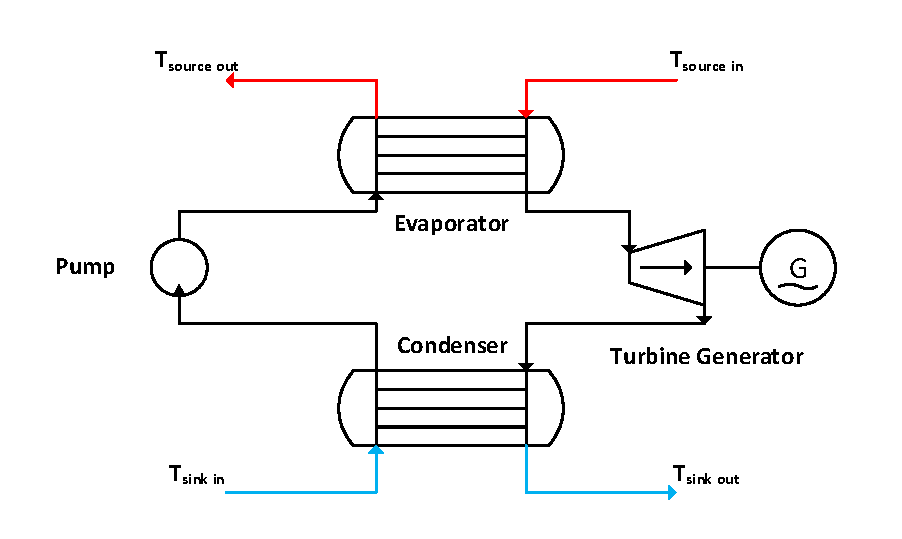
\includegraphics[width=\textwidth]{figures/RankineCycleDiagram.pdf}

	\caption{Diagram of a Rankine cycle system.}
	\label{fig:rankine_cycle_diagram}
	
\end{figure}

For geothermal sources, generally high enthalpy systems can be implemented directly with a single loop using the flash or dry steam processes. However, for lower enthalpy systems, water cannot be used as a working fluid because the temperatures are not high enough to vaporize it. In these cases an organic Rankine cycle, which uses an organic working fluid such as refrigerants instead of water, can be employed. Working fluids are typically selected for relatively low vaporization temperatures, but the thermodynamic states of the heat source must also be considered. The selection of the type of expander and pumps are discussed in Kreider \cite{Kreider}. Generally larger diameter expanders operate at lower speeds.




%\subsection{Pilgrim Hot Springs}
%Do this in 1st chapter not conv/geotherm chapter
%More thourough description of the resource and potential development plans.

 %used to contain geothermal chapter, now contains thermal section

\section{Electric Conversion}

%\subsection{Linear Power Supplies}
%Linear

%\subsection{Switched Mode Power Supplies}

\subsection{PWM vs PFM}

\subsection{DC-DC}
recent developments

\subsection{Rectifiers}
recent developments

\subsection{Inverters}
recent developments

%%This file used to contain the geothermal chapter, now contains thermal/mechanical section of the conversion chapter
\section{Thermal Energy}
Thermal energy, or heat, can originate from many different sources including combustion of a fuel, radioactive decay, or absorption of light from the sun. Heat can be used directly to warm a building, but it is also a critical step in most traditional methods of generating electrical power. 
%\chapter{Geothermal Energy}
%\label{ch:geothermal}

\subsection{Enthalpy}
Enthalpy describes the energy of a system available to be converted to work. It is related to the temperature of the geothermal resource, but also dependent on the pressure and volume. Temperature is usually the primary metric of a resource, but even a high temperature source is useless without sufficient volume flow. Quantitatively enthalpy is expressed as \cite{Nellis2009}
\begin{equation}
H = U + pV
\end{equation}
where $U$ is the internal energy, which is function of temperature, $p$ is the pressure of the system, and $V$ is the volume. Generally it is more convenient to use the change in enthalpy rather than absolute values. After a system undergoes some thermodynamic process, the system will always have some remaining internal energy, pressure, and volume. Therefore, a change in enthalpy better describes the energy extracted from (or absorbed by) the system.
Additionally, the enthalpy of a system is often normalized by the its mass for comparison to other sized systems and the mass specific enthalpy, $h$, is used instead.
\nomenclature[V]{$H$}{Enthalpy of a fluid\nomunit{\si{\joule}}}
\nomenclature[V]{$U$}{Internal energy of a fluid\nomunit{\si{\joule}}}
\nomenclature[V]{$p$}{Aboluete fluid pressure\nomunit{\si{\pascal}}}
\nomenclature[V]{$V$}{Fluid volume\nomunit{\si{\meter\cubed}}}
\nomenclature[V]{$h$}{Mass specific enthalpy of a fluid\nomunit{\si{\joule\per\kilogram}}}


\subsection{Geothermal Cycles}
%%Describe each of the following but focus on cycles for low enthalpy sources
Geothermal systems can be classified as high-, medium-, or low-enthalpy\footnote{While the technical definitions differ, the terms enthalpy, heat, and temperature are often used interchangeably when qualitatively describing geothermal sources.}. Although there is no formal delineation, high-enthalpy sources generally have temperatures greater than about $150$ \textcelsius{} ($302$ \textdegree{}F) and low-enthalpy sources have temperatures lower than $100$ \textcelsius{} ($212$ \textdegree{}F) \cite{Norden2011}. Depending on the amount of extractable energy of the resource, different geothermal processes or cycles can be used to extract the maximum amount of energy from the resource.

\subsubsection{Dry Steam}
This high-enthalpy processes extracts hot steam from the earth. The steam is sent directly through a turbine then condensed into liquid water and injected back underground. 

\subsubsection{Flash Steam} 
In the flash steam process high pressure hot water is extracted then, allowed to boil becoming steam and low pressure hot water. The steam is sent through a turbine then condensed, recombined with water, and injected back underground.

\subsubsection{Binary Cycle} 
As the name implies, binary cycles involve two loops: a heat source loop and working fluid loop. Heat is collected in the heat source loop and transferred to the working loop through a heat exchanger. The working fluid then undergoes the vaporization process to spin a turbine or other type of expander. The expander is connected to a generator which converts the rotational mechanical energy into electrical energy. After some of the heat is converted, the working fluid passes through a condenser where it is cooled further. Sometimes the cooling process involves drawing in air at ambient temperature, but it can also involve a third loop. The fluids within each of the cycles must be moved using pumps. The pumps themselves need to be powered and act as a parasitic load to the system.

Binary cycles are not limited to low or medium enthalpy heat sources. The most common binary cycle is the Rankine Cycle. A diagram of the process can be seen in \autoref{fig:rankine_cycle_diagram}. In an ideal Rankine Cycle heat is added to the working fluid under high pressure to change its phase from liquid to gas. The fluid expands isentropically\footnote{In thermodynamics, isentropic processes do not have a net change in entropy.} which rotates the generator shaft, causing the fluid's temperature and pressure to drop. Additional heat is then expelled from the fluid as it condenses at a constant low pressure side of the system. Finally the fluid is isentropically pumped back to the high pressure and the process begins again.
\begin{figure}[h]
	\centering

	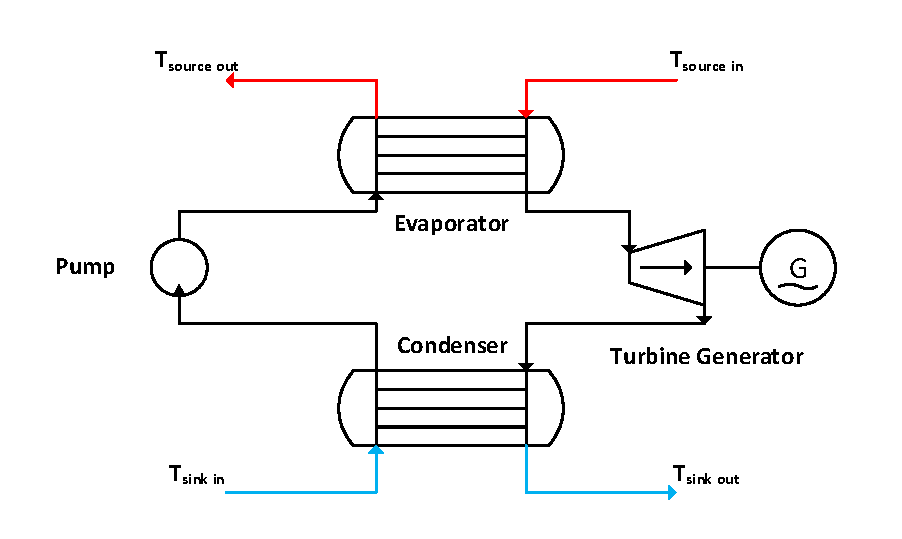
\includegraphics[width=\textwidth]{figures/RankineCycleDiagram.pdf}

	\caption{Diagram of a Rankine cycle system.}
	\label{fig:rankine_cycle_diagram}
	
\end{figure}

For geothermal sources, generally high enthalpy systems can be implemented directly with a single loop using the flash or dry steam processes. However, for lower enthalpy systems, water cannot be used as a working fluid because the temperatures are not high enough to vaporize it. In these cases an organic Rankine cycle, which uses an organic working fluid such as refrigerants instead of water, can be employed. Working fluids are typically selected for relatively low vaporization temperatures, but the thermodynamic states of the heat source must also be considered. The selection of the type of expander and pumps are discussed in Kreider \cite{Kreider}. Generally larger diameter expanders operate at lower speeds.




%\subsection{Pilgrim Hot Springs}
%Do this in 1st chapter not conv/geotherm chapter
%More thourough description of the resource and potential development plans.

	%Electronic conversion and thermal/mechanical conversion chapters combined
\chapter{Model Validation and Simulation}
\label{ch:model}

The model attempts to recreate a microgrid which uses some form of DER as a primary power source along side energy storage in order power the load. \autoref{fig:abridged_flow_diagram} shows a simplified flow diagram of the model using an ORC for the DER. The components include a ORC as a source, a load, a form of energy storage, and an inverter to link the energy storage with other pieces. The ORC block is made up of heat exchangers, an isentropic pump, an isentropic exapnder, and an induction generator. The load block \verb|one line description of load|. The energy storage block \verb|one line description of energy storage|. The inverter block \verb|one line description of inverter|.

\begin{figure}[h]
	\centering
	\caption{A simplified diagram of power and data flows of the model. Blue lines represent electrical power connections and flows similar to a one-line diagram. Green boxes represent data flow from one part of the model to another.}
	\label{fig:abridged_flow_diagram_label}
	
	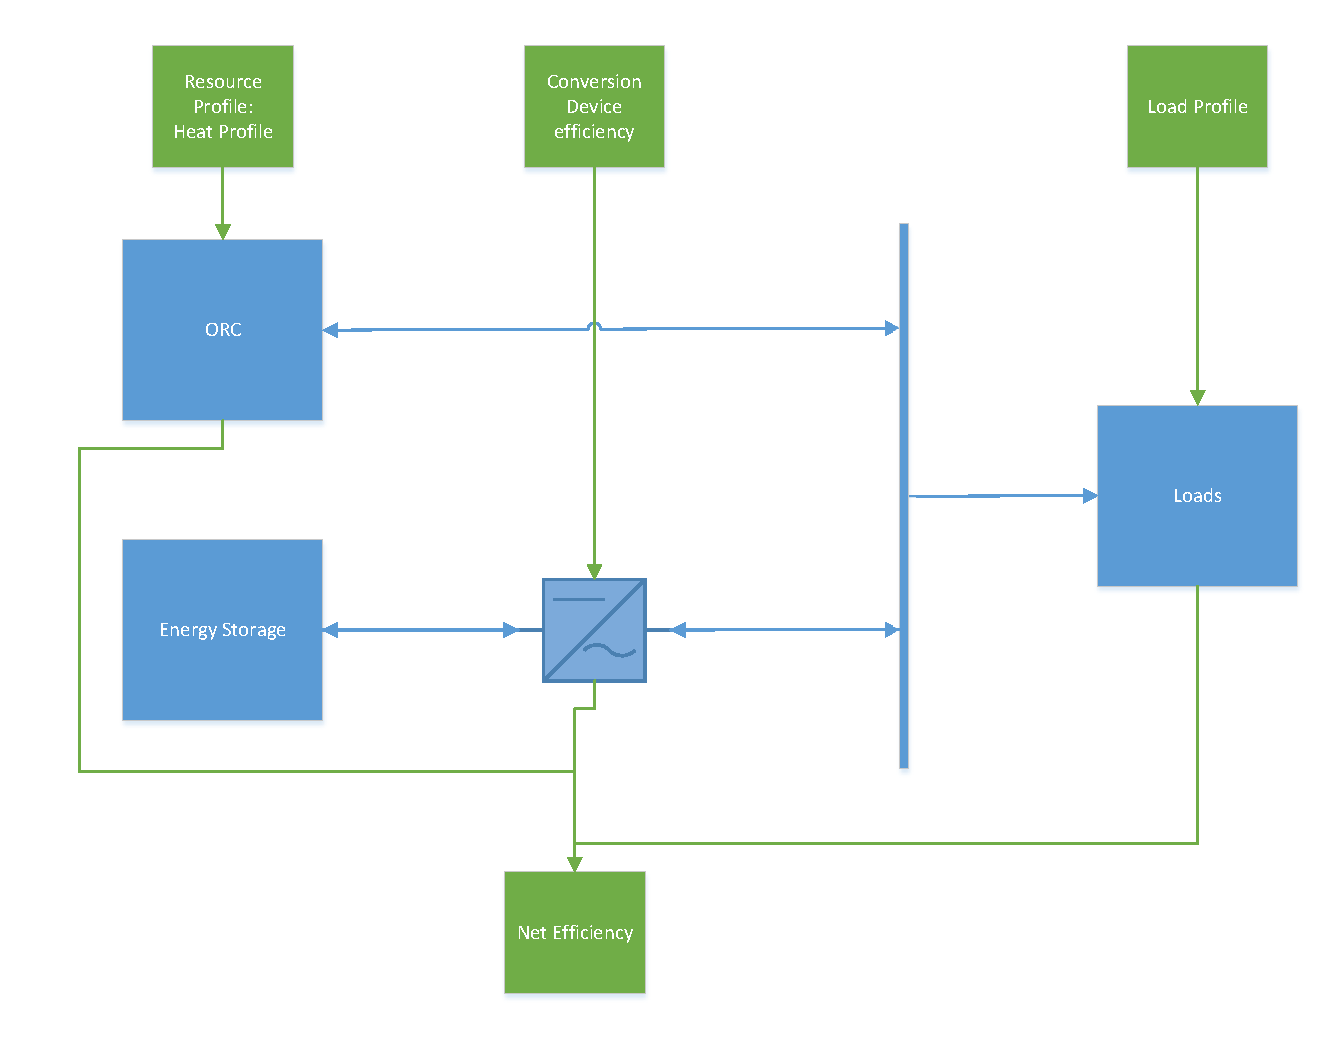
\includegraphics[width=\textwidth]{figures/Abridged Pilgrim Model Flow diagram - AC bus.pdf} 
	%\includegraphics[width=\textwidth]{figures/SimpleFlowDiagram.pdf}

\end{figure}
\chapter{ORC System Model Validation, Analysis, and Case Study Results}
\label{ch:analysis}

With the ORC prime power system model constructed as described in \autoref{ch:model}, simulations can be conducted to validate it and verify the model simulates a system as expected. After validation, two case studies, a greenfield and brownfield microgrid, can be investigated and analyzed in order to determine whether geothermal organic Rankine cycle generators can be viably used as primary power sources.

\section{Validation}
%Before simulating  the greenfield and brown field case study scenarios, the model needs to be validated. 
The model validation is conducted by comparing the results of an ORC test with the simulation results under similar conditions. The test, performed in 2013, is from the University of Alaska Fairbanks and is documented in a report by Lin et al. \cite{Lin2014}. The report details the process of testing an Electratherm Green Machine ORC system in a controlled environment at the UAF power plant.
%and in the field for waste heat reclamation of a diesel generator at the Tok, Alaska powerhouse.

During the sizing of the ORC system turbine, $\eta_{turbine}$, and pump, $\eta_{pump}$, efficiencies as well as heat exchanger areas, $A_{evap}$ and $A_{cond}$, and transfer coefficients, $U_{evap}$ and $U_{cond}$, were assumed based off of published values and conventional practice, but final values were not reported. These assumed values are used as the input of the model. All of the non-variable ORC prime power system parameters for the validation can be seen in \autoref{tab:verification_ORC_params}.
\begin{table}%[h]
	\centering
	\caption{Input parameters for the validation of the ORC prime power system model.}
	%\rowcolors{5}{}{gray!10}
	\label{tab:verification_ORC_params}
	\begin{tabular}{rl}
		\toprule
		           Parameter & Value                                        \\ \midrule
		         $U_{evap}$ & 1500 \si{\watt\per\kelvin\per\meter\squared} \\
		         $A_{evap}$ & 26.5 \si{\meter\squared}                     \\
		         $U_{cond}$ & 1400 \si{\watt\per\kelvin\per\meter\squared} \\
		         $A_{cond}$ & 102.5 \si{\meter\squared}                    \\
		    $\eta_{turbine}$ & 0.78                                         \\
		       $\eta_{pump}$ & 0.7                                          \\
		$\eta_{pump\ driver}$ & 0.9                                          \\
		   $\eta_{inverter}$ & 1.0                                          \\ \bottomrule
	\end{tabular}
\end{table}


The only reported electrical parameters of the three-phase induction generator were the frequency (\SI{60}{\hertz}) and the line to line voltage (\SI{480}{\volt} AC). The impedance parameters were taken from a 10 HP machine in \cite{Ouazenne1983} and scaled based off the expected relative power output. The external excitation capacitance, $C_x$, was selected in order to yield a terminal voltage roughly equal to the rated voltage. The impedance parameters can be seen in \autoref{tab:verification_SCIG_params}.
% and the magnetization curve comparing internal voltage, $E$, and the magnetizing reactance at rated frequency, $X_m$, can be seen in Fig X.
\begin{table}%[h]
	\centering
	\caption{Input generator parameters for the validation of the organic Rankine cycle prime power system model.}
	%\rowcolors{5}{}{gray!10}
	\label{tab:verification_SCIG_params}
	\begin{tabular}{rl}
		\toprule
		    Parameter & Value                                       \\ \midrule
		      $poles$ & 4                                           \\
		  $f_{rated}$ & $\SI{60}{\hertz}$                           \\
		        $R_s$ & $\SI{0.0279}{\ohm}$                         \\
		        $X_s$ & $\SI{0.0798}{\ohm}$                         \\
		        $R_r$ & $\SI{0.0272}{\ohm}$                         \\
		        $X_r$ & $\SI{0.0475}{\ohm}$                         \\
		        $C_x$ & $\SI{1000}{\micro\farad}$                   \\
		    $R_{esr}$ & $\SI{0}{\ohm}$                              \\
		 $K_{bering}$ & $\SI{0.5}{\kilo\watt\per\second}$           \\
		$K_{windage}$ & $\SI{0.003}{\kilo\watt\per\second\squared}$ \\ \bottomrule
	\end{tabular}
\end{table}

%\input{figures/magCurve}

Four loads were simulated under different combinations of heat sink flow rates and heat source temperatures and flow rates, as well as high and low pressure values as shown in  \autoref{tab:verification_ORC_vars}. For the validation process, pressure values were measured, but not explicitly detailed. Instead, pressure ranges were reported, so estimated values within the ranges were used for the model. The working fluid flow rate could not be used as an input to the model because it was also not reported. Instead the model uses load power set points such that the gross power produced by the simulation approximately matches the reported value and returns the necessary working fluid flow rate to achieve that power output.  
\begin{table}[h]
	\centering
	\caption{Input variables for the validation of the organic Rankine cycle prime power system model.}
	%\rowcolors{5}{}{gray!10}
	\label{tab:verification_ORC_vars}
	\begin{tabular}{rllll}
		\toprule
		                                              &  Test &       &       &       \\ \cline{2-5}
		                                              &     1 &     2 &     3 &     4 \\ \midrule
		$T_{source\ in}(\si{\kelvin})$                & 363.9 & 363.6 & 353.0 & 353.9 \\
		$T_{sink\ in}(\si{\kelvin})$                  & 283.5 & 284.6 & 283.6 & 284.6 \\
		$\dot{m}_{source}(\si{\kilogram\per\second})$ &  18.3 &  7.28 &  18.4 &  7.35 \\
		$\dot{m}_{sink}(\si{\kilogram\per\second})$   &  13.0 &  7.53 &  13.0 &  7.54 \\
		$p_{hi}(\si{\kilo\pascal})  $                 &  0.68 &  0.75 &  0.60 &  0.60 \\
		$p_{low}(\si{\kilo\pascal}) $                 &  0.14 &  0.17 &  0.14 &  0.16 \\
		$P_{setpoint}(\si{\kilo\watt})$               &  35.7 &  26.0 &  25.0 &  19.0 \\ 
		\bottomrule
	\end{tabular}
\end{table}



The mechanical power, $P_{mech}$, the generator power, $P_{gen}$, inverter output power, $P_{out}$, and the electrical power consumed by the pump, $P_{pump}$ of the four tests are plotted in \autoref{fig:verificationPower01}. \autoref{fig:verificationHeat01} plots the heat flows though the evaporator, $\dot{Q}_{evap}$, and condenser,  $\dot{Q}_{cond}$. The inlet and outlet temperatures of the source, $T_{source\ in}$ and $T_{source\ out}$, and sink, $T_{sink\ in}$ and $T_{sink\ out}$ are plotted in \autoref{fig:verificationWaterTemp01}. \autoref{tab:verification_results01} compares simulated values in the plots with the measured values from the report.
\begin{table}[h]
	\centering
	\caption{Comparison of output variables for the validation of the ORC prime power system model.}
	%\rowcolors{5}{}{gray!10}
	\label{tab:verification_results01}
	\begin{tabular}{rllllllll}
		\toprule
		                                      & Test  &       &       &       &       &       &       &         \\ \cline{2-9}
		                                      & 1     &       & 2     &       & 3     &       & 4     &         \\
		                                      & Meas. & Model & Meas. & Model & Meas. & Model & Meas. & Model   \\ \midrule
		           $P_{out}(\si{\kilo\watt})$ & 40.7  & 40.6  & 31.8  & 31.6  & 29.2  & 29.2  & 22.7  & 23.0    \\
		          $P_{pump}(\si{\kilo\watt})$ & 2.6   & 4.9   & 1.9   & 5.6   & 1.5   & 4.1   & 1.3   & 4.2     \\
		   %$P_{source pump}(\si{\kilo\watt})$ & 9.6   & -     & 1.0   & -     & 10.0  & -     & 1.0   & -       \\
		     %$P_{sink pump}(\si{\kilo\watt})$ & 3.5   & -     & 1.0   & -     & 3.5   & -     & 1.0   & -       \\
  $\dot{Q}_{evap}(\si{\kilo\watt}_\text{th})$ & 519   & 621   & 413   & 540   & 393   & 540   & 328   & 466     \\
  $\dot{Q}_{cond}(\si{\kilo\watt}_\text{th})$ & 464   & 583   & 385   & 512   & 356   & 514   & 303   & 446     \\
		      $T_{source\ out}(\si{\kelvin})$ & 357.2 & 355.8 & 350.1 & 345.9 & 347.9 & 346.0 & 342.0 & 337.5   \\
		        $T_{sink\ out}(\si{\kelvin})$ & 292.1 & 294.2 & 296.9 & 300.9 & 290.1 & 293.0 & 294.2 & 298.7   \\ \bottomrule
		      %$P_{setpoint}(\si{\kilo\watt})$ &       &       &       &       &       &       &       &         \\
    %$\dot{m}_{wf}(\si{\kilogram\per\second})$ & -     &       & -     &       & -     &       & -     &         \\ 
\end{tabular}
\end{table}


\begin{figure}[p]
	\centering
	
	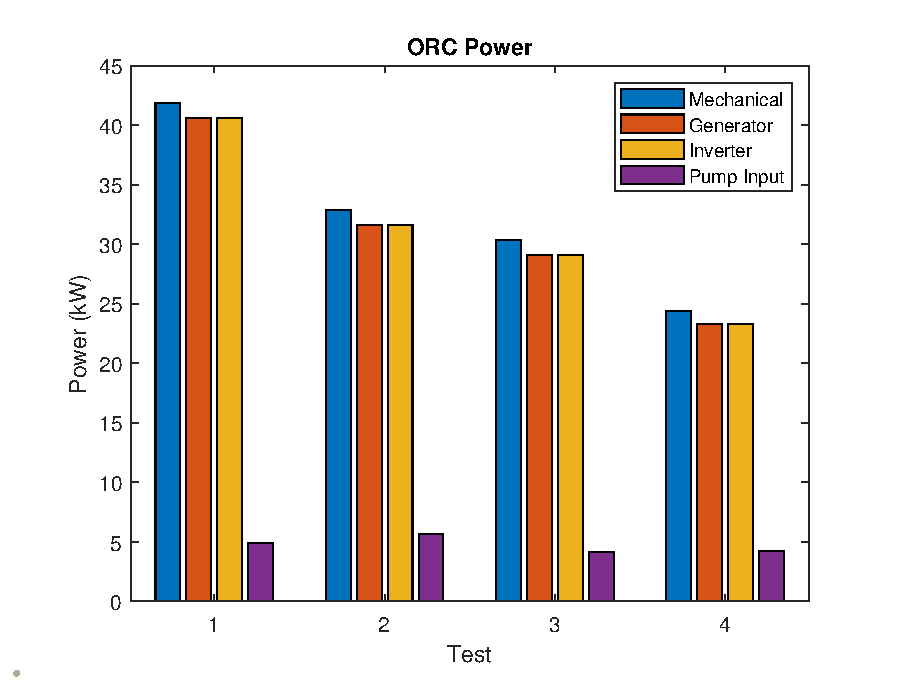
\includegraphics[width=\textwidth]{figures/VerificationPower01}
	%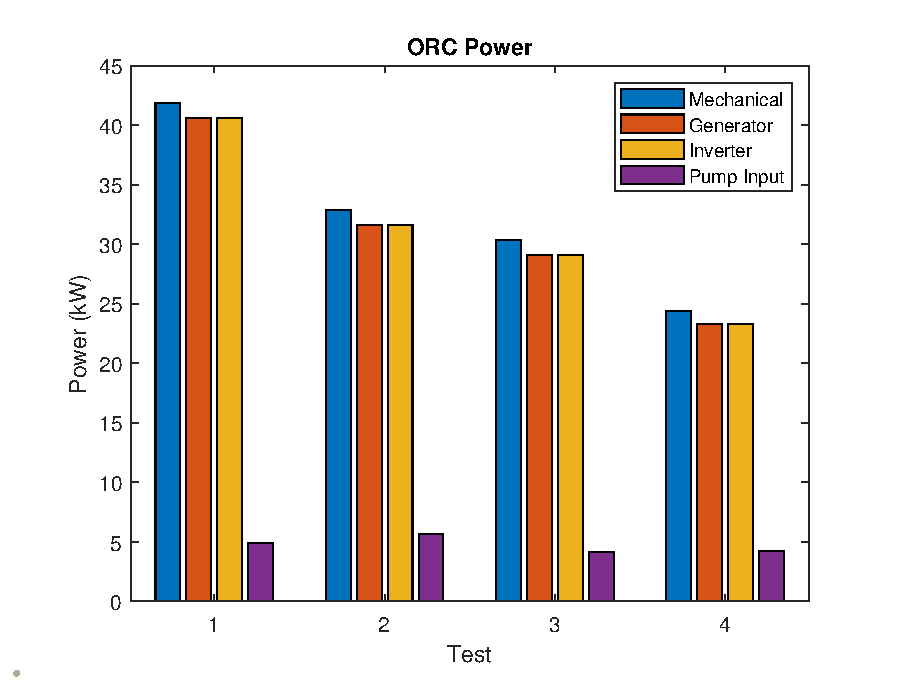
\includegraphics[width=0.5\textwidth]{figures/VerificationPower01}
	
	\caption{Comparison of mechanical power, generator power, inverter output power, and pump power consumption for the validation of the ORC prime power system model. All tests assume a sink temperature of \SI{283}{\kelvin} (\SI{10}{\degreeCelsius}). Tests 1 and 2 use a heat source temperature of \SI{364}{\kelvin} (\SI{91}{\degreeCelsius}), while tests 3 and 4 use \SI{353}{\kelvin} (\SI{79}{\degreeCelsius}). Tests 1 and 3 use a source flow rate of \SI{19}{\liter\per\second} and a sink flow rate of \SI{13}{\liter\per\second}, where as tests 3 and 4 use a source and sink flow rate of \SI{8}{\liter\per\second}.
	%The power setpoints of the four tests are \SIlist{27.5;40.0;30.8;42.0}{\kilo\watt}. Tests 1 and 3 use the maximum power setpoint while also ensuring the working fluid fully evaporates in the evaporator. Tests 2 and 4, use the maximum power setpoint while maintaining a stable simulation. 
	}
	%Psetpoint[2.75e4;4.0e4;3.08e4;4.2e4;]
	\label{fig:verificationPower01}
\end{figure}
\begin{figure}[h]
	\centering
	
	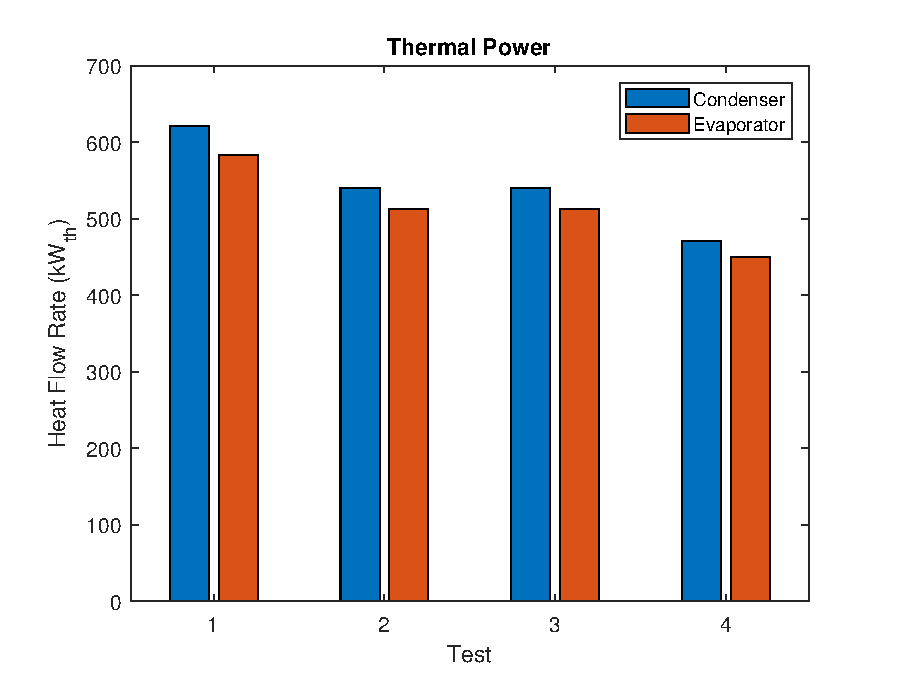
\includegraphics[width=\textwidth]{figures/VerificationHeat01}
	%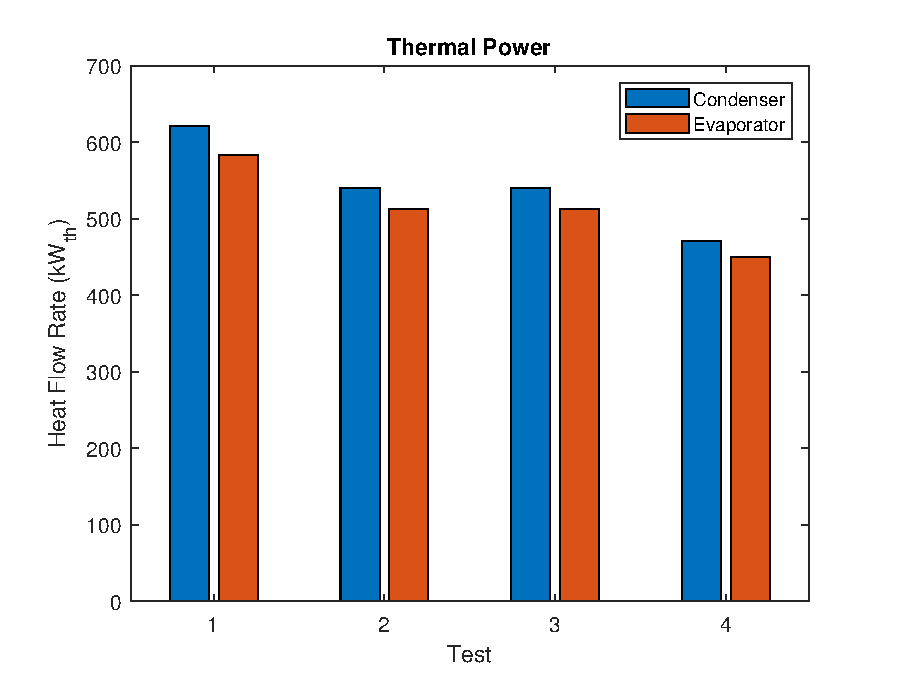
\includegraphics[width=0.5\textwidth]{figures/VerificationHeat01}
	
	\caption{Comparison of evaporator and condenser heat flow rates for the validation of the ORC prime power system model. All tests assume a sink temperature of \SI{283}{\kelvin} (\SI{10}{\degreeCelsius}). Tests 1 \& 2 use a heat source temperature of \SI{364}{\kelvin} (\SI{91}{\degreeCelsius}), while tests 3 \& 4 use \SI{353}{\kelvin} (\SI{79}{\degreeCelsius}). Tests 1 \& 3 use a source flow rate of \SI{19}{\liter\per\second} and a sink flow rate of \SI{13}{\liter\per\second}, where as test 3 \& 4 use a source and sink flow rate of \SI{8}{\liter\per\second}.
	%The power setpoints of the four tests are \SIlist{27.5;40.0;30.8;42.0}{\kilo\watt}. Tests 1 \& 3 use the maximum power setpoint while also ensuring the working fluid fully evaporates in the evaporator. Tests 2 \& 4, use the maximum power setpoint while maintaining a stable simulation. 
	}
	%Psetpoint[2.75e4;4.0e4;3.08e4;4.2e4;]
	\label{fig:verificationHeat01}
\end{figure}
\begin{figure}[p]
	\centering
	
	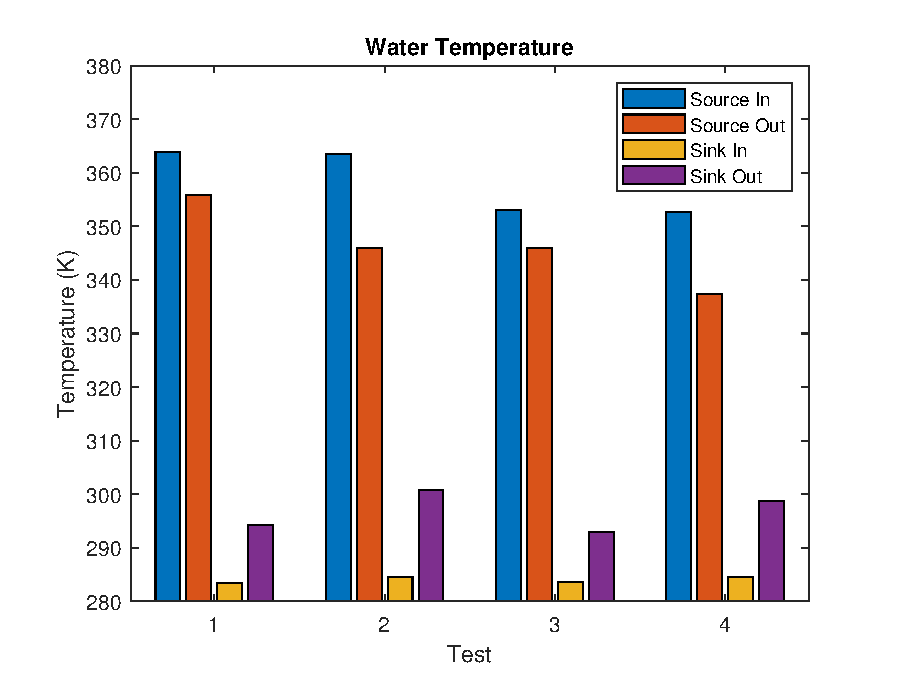
\includegraphics[width=\textwidth]{figures/VerificationWaterTemp01}
	%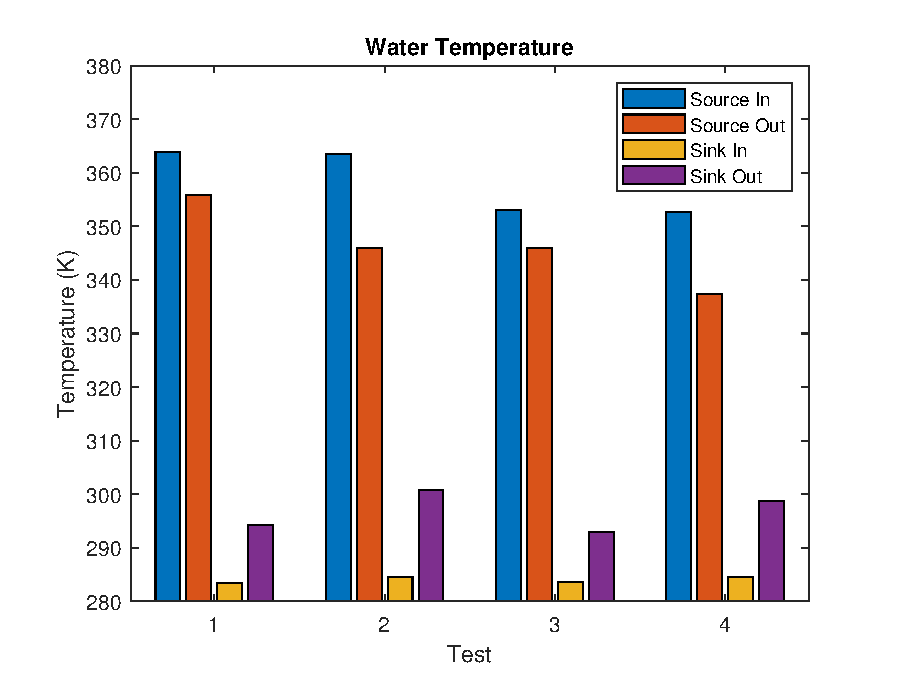
\includegraphics[width=0.5\textwidth]{figures/VerificationWaterTemp01}
	
	\caption{Comparison of source and sink inlet and outlet temperatures for the validation of the ORC prime power system model. All tests assume a sink temperature of \SI{283}{\kelvin} (\SI{10}{\degreeCelsius}). Tests 1 and 2 use a heat source temperature of \SI{364}{\kelvin} (\SI{91}{\degreeCelsius}), while tests 3 and 4 use \SI{353}{\kelvin} (\SI{79}{\degreeCelsius}). Tests 1 and 3 use a source flow rate of \SI{19}{\liter\per\second} and a sink flow rate of \SI{13}{\liter\per\second}, where as tests 3 and 4 use a source and sink flow rate of \SI{8}{\liter\per\second}.
	%The power setpoints of the four tests are \SIlist{27.5;40.0;30.8;42.0}{\kilo\watt}. Tests 1 and 3 use the maximum power setpoint while also ensuring the working fluid fully evaporates in the evaporator. Tests 2 and 4, use the maximum power setpoint while maintaining a stable simulation. 
	}
	%Psetpoint[2.75e4;4.0e4;3.08e4;4.2e4;]
	\label{fig:verificationWaterTemp01}
\end{figure}

As desired, the gross electrical power output of the model matches the measured value for each set of inputs. However, the power consumed to run the pump is a factor of 2-3 times greater in the model than what was measured. A pump sizing guide \cite{CheGuide2017} was used to calculate hypothetical hydraulic power needed to move a liquid at the density of R245-fa across each of the pressure differences listed at the corresponding flow rates. When these hydraulic power values have the assumed pump and drive efficiencies applied as well, they match the pump power values of the model. This indicates the working fluid flow rates of the model are much greater than the operating values measured during the Green Machine ORC system test.

The calculated heat transferred in both the evaporator and the condenser are greater than what was measured in each case. Although the values do tend to follow a similar pattern with higher source temperatures and water flow rates resulting in greater rates of heat transferred. Additionally, the source and sink fluids undergo a greater temperature change in the model as a result of the higher heat flow rates.


%The likely reason for the difference in heat flows is model assumes all the heat flows from one fluid to another and does not affect the ambient temperature. This is also a possible explanation for higher pump power consumptions seen in the model. With both more heat being added and removed from the working fluid, but the same amount of mechanical power being extracted from it, the fluid is likely being 

Pressure was plotted against enthalpy at various points of the cycle in \autoref{fig:verifcation_ph01} for each of the four tests. The two curves indicate the pressure-enthalpy combinations of R245-fa where the working fluid begins to condense and vaporize. The top-left group of points represents the working fluid at the outlet of the pump. The top-right group represents the working fluid at the inlet of the expander. The bottom-right group represents the working fluid at the outlet of the expander. Finally, The bottom-left group represents the working fluid at the inlet of the pump.
\begin{figure}[h]
	\centering

	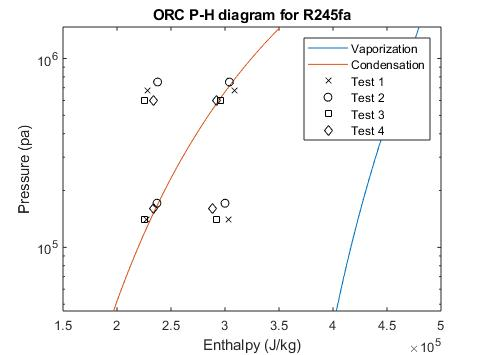
\includegraphics[width=\textwidth]{figures/VerificationPH01}
	%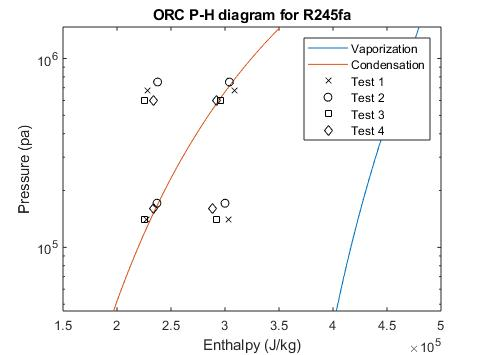
\includegraphics{figures/VerificationPH01}

	\caption{Pressure-Enthalpy plot of R245-fa for ORC verification. 
	For tests 1 \& 2 $T_{source}$ is about \SI{364}{\kelvin} (\SI{195}{\degreeFahrenheit})
	while for 3 \& 4 $T_{source}$ is \SI{353}{\kelvin} (\SI{175}{\degreeFahrenheit}). 
	In all cases $T_{sink}$ is about \SI{283}{\kelvin} (\SI{50}{\degreeFahrenheit}). 
	The hot water flow rate for tests 1 \& 3 are \SI{18.9}{\liter\per\second} (\SI{300}{\gpm})
	and	\SI{7.6}{\liter\per\second} (\SI{120}{\gpm}) for test 2 \& 4. 
	The cold water flow rate for tests 1 \& 3 are \SI{12.6}{\liter\per\second} (\SI{200}{\gpm})
	and \SI{7.6}{\liter\per\second} (\SI{120}{\gpm}) for test 2 \& 4.}
	\label{fig:verifcation_ph01}
\end{figure}

For each of these tests, the working fluid just barely begins to boil in the evaporator, if at all. It is expected that the working fluid will either completely vaporize, or at least be further to the right in the liquid-vapor region. Along with the higher than expected pump power, this also indicates that there is more working fluid being pumped throughout the cycle in the model than what was measured.

To re-create conditions where the system outputs comparable between the modeled and measured values while pumping less fluid, the evaporator area is increased by a factor of four so it is comparable to the area of the condenser. Additionally, the pressure set points are adjusted to values seen in \autoref{tab:verification_ORC_vars02} to account for the new temperatures of the working fluid.
\begin{table}%[h]
	\centering
	\caption{Input variables for the verification of the Organic Rankine Cycle Model.}
	%\rowcolors{5}{}{gray!10}
	\label{tab:verification_ORC_vars02}
	\begin{tabular}{rllll}
		\toprule
		                                              &  Case &       &       &       \\ \cline{2-5}
		                                              &     1 &     2 &     3 &     4 \\ \midrule

		$p_{hi}(\si{\kilo\pascal})  $                 &  0.68 &  0.75 &  0.60 &  0.60 \\
		$p_{low}(\si{\kilo\pascal}) $                 &  0.14 &  0.17 &  0.14 &  0.16 \\
%		$P_{setpoint}(\si{\kilo\watt})$               &  34.7 &  27.1 &  24.6 &  19.0 \\ 
		\bottomrule
	\end{tabular}
\end{table}



The results of the second set of validation tests are plotted in \autoref{fig:verificationPower02} for the power values, \autoref{fig:verificationHeat02} for the heat flow rate values, and \autoref{fig:verificationWaterTemp02} for the water temperature values. \autoref{tab:verification_results02} compares the simulation results with the measured results. As expected, the gross output power remained roughly equal to the measured values. The consumed pump power decreased significantly in the new set of tests. Those values are now about half the measured ones, indicating the fluid is moving at a slower rate. The thermal power measurements are now greater than the simulated values by about \SIrange{30}{80}{\kilo\watt\textsubscript{th}} and the source and sink outlet temperatures are correspondingly higher and lower, respectively. \autoref{fig:verifcation_ph02} shows the lower mass flow rate of the working fluid allows it to fully vaporize due to the larger transfer area of the evaporator. 
\begin{table}%[h]
	\centering
	\caption{Comparison of output variables for the verification of the ORC Model with modified evaporator area.}
	%\rowcolors{5}{}{gray!10}
	\label{tab:verification_results02}
	\begin{tabular}{rllllllll}
		\toprule
		                                           & Case  &       &       &       &       &       &       &       \\ \cline{2-9}
		                                           & 1     &       & 2     &       & 3     &       & 4     &       \\
		                                           & Meas. & Model & Meas. & Model & Meas. & Model & Meas. & Model \\ \midrule
		              $P_{gross}(\si{\kilo\watt})$ & 40.7  & 40.7  & 31.8  & 31.9  & 29.2  & 29.2  & 22.7  & 22.5  \\
		               $P_{pump}(\si{\kilo\watt})$ & 2.6   & 1.1   & 1.9   & 0.92  & 1.5   & 0.72  & 1.3   & 0.55  \\
		            %$P_{source}(\si{\kilo\watt})$ & 9.6   & -     & 1.0   & -     & 10.0  & -     & 1.0   & -     \\
		              %$P_{sink}(\si{\kilo\watt})$ & 3.5   & -     & 1.0   & -     & 3.5   & -     & 1.0   & -     \\
		              $P_{evap.}(\si{\kilo\watt})$ & 519   & 441   & 413   & 340   & 393   & 364   & 328   & 277   \\
		              $P_{cond.}(\si{\kilo\watt})$ & 464   & 400   & 385   & 307   & 356   & 335   & 303   & 254   \\
		            $T_{source,out}(\si{\kelvin})$ & 357.2 & 358.2 & 350.1 & 352.5 & 347.9 & 348.2 & 342.0 & 343.7 \\
		              $T_{sink,out}(\si{\kelvin})$ & 292.1 & 290.9 & 296.9 & 294.4 & 290.1 & 289.7 & 294.2 & 292.6 \\ \bottomrule
		          %$P_{setpoint}(\si{\kilo\watt})$ &       &       &       &       &       &       &       &       \\
		%$\dot{m}_{wf}(\si{\kilogram\per\second})$ & -     &       & -     &       & -     &       & -     &
	\end{tabular}
\end{table}


\begin{figure}[h]
	\centering
	
	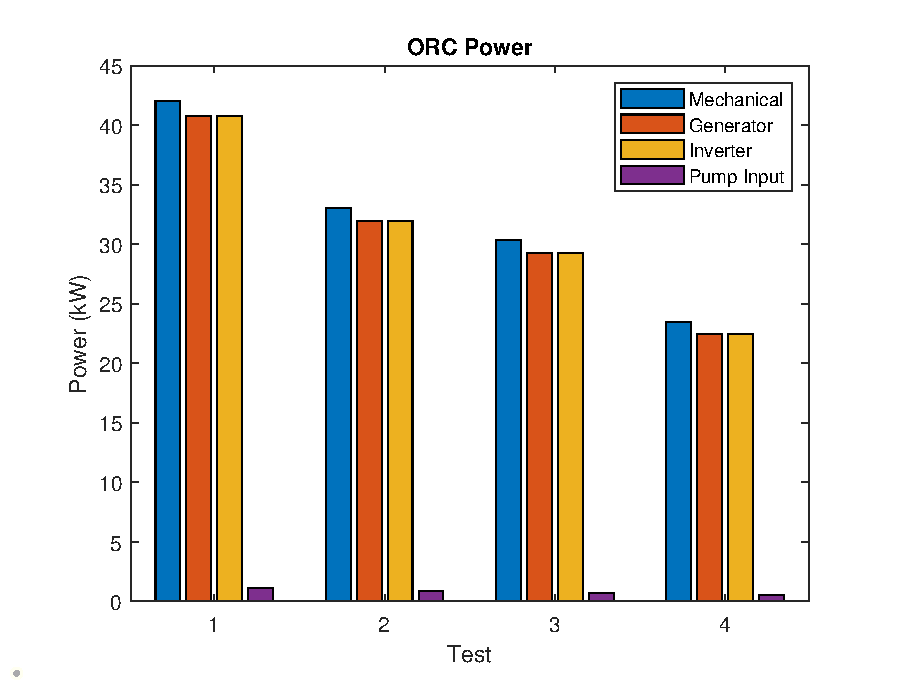
\includegraphics[width=\textwidth]{figures/VerificationPower02}
	%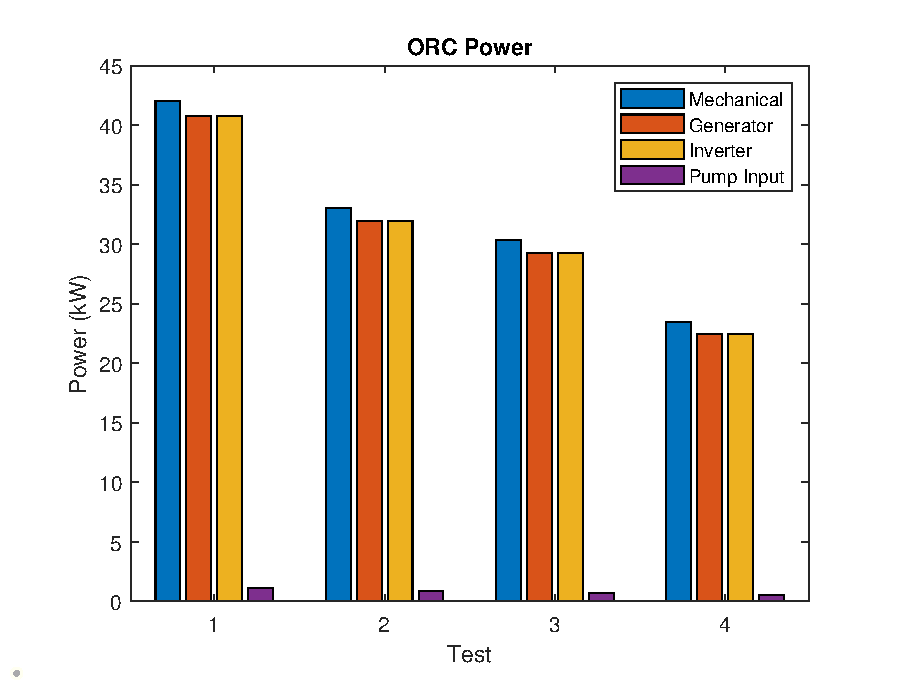
\includegraphics[width=0.5\textwidth]{figures/VerificationPower02}
	
	\caption{Comparison of mechanical power, generator power, inverter output power, and pump power consumption for the validation of the ORC prime power system model with an increased evaporator area. All tests assume a sink temperature of \SI{283}{\kelvin} (\SI{10}{\degreeCelsius}). Tests 1 \& 2 use a heat source temperature of \SI{364}{\kelvin} (\SI{91}{\degreeCelsius}), while tests 3 \& 4 use \SI{353}{\kelvin} (\SI{79}{\degreeCelsius}). Tests 1 \& 3 use a source flow rate of \SI{19}{\liter\per\second} and a sink flow rate of \SI{13}{\liter\per\second}, where as test 3 \& 4 use a source and sink flow rate of \SI{8}{\liter\per\second}.
	%The power setpoints of the four tests are \SIlist{27.5;40.0;30.8;42.0}{\kilo\watt}. Tests 1 \& 3 use the maximum power setpoint while also ensuring the working fluid fully evaporates in the evaporator. Tests 2 \& 4, use the maximum power setpoint while maintaining a stable simulation. 
	}
	%Psetpoint[2.75e4;4.0e4;3.08e4;4.2e4;]
	\label{fig:verificationPower02}
\end{figure}
\begin{figure}[p]
	\centering
	
	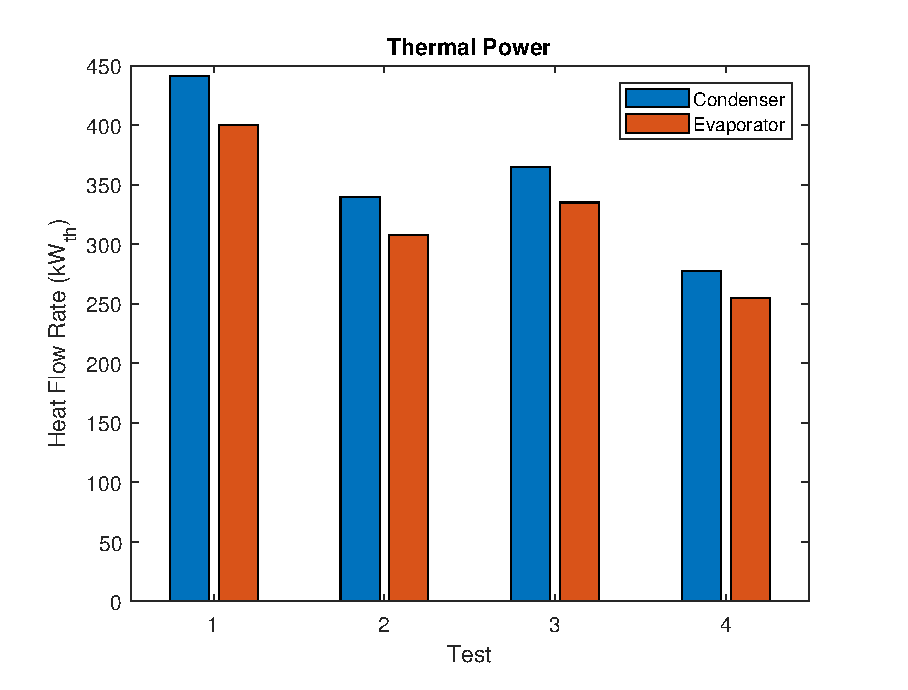
\includegraphics[width=\textwidth]{figures/VerificationHeat02}
	%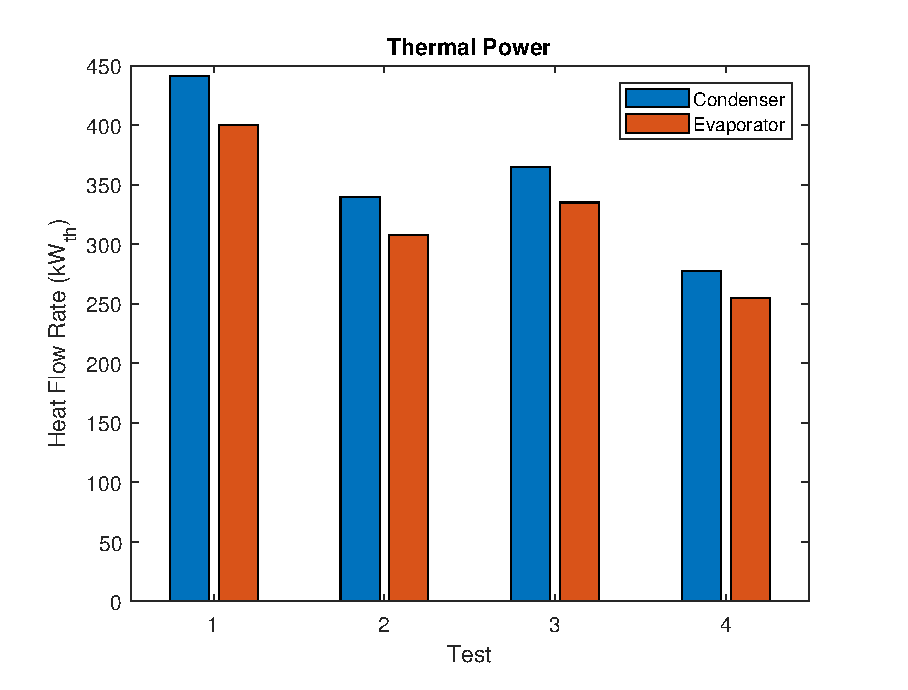
\includegraphics[width=0.5\textwidth]{figures/VerificationHeat02}
	
	\caption{Comparison among evaporator and condenser heat flow rates for the validation of the ORC prime power system model with an increased evaporator area. All tests assume a sink temperature of \SI{283}{\kelvin} (\SI{10}{\degreeCelsius}). Tests 1 and 2 use a heat source temperature of \SI{364}{\kelvin} (\SI{91}{\degreeCelsius}), while tests 3 and 4 use \SI{353}{\kelvin} (\SI{79}{\degreeCelsius}). Tests 1 and 3 use a source flow rate of \SI{19}{\liter\per\second} and a sink flow rate of \SI{13}{\liter\per\second}, where as tests 3 and 4 use a source and sink flow rate of \SI{8}{\liter\per\second}.
	%The power setpoints of the four tests are \SIlist{27.5;40.0;30.8;42.0}{\kilo\watt}. Tests 1 and 3 use the maximum power setpoint while also ensuring the working fluid fully evaporates in the evaporator. Tests 2 and 4, use the maximum power setpoint while maintaining a stable simulation. 
	}
	%Psetpoint[2.75e4;4.0e4;3.08e4;4.2e4;]
	\label{fig:verificationHeat02}
\end{figure}
\begin{figure}[h]
	\centering
	
	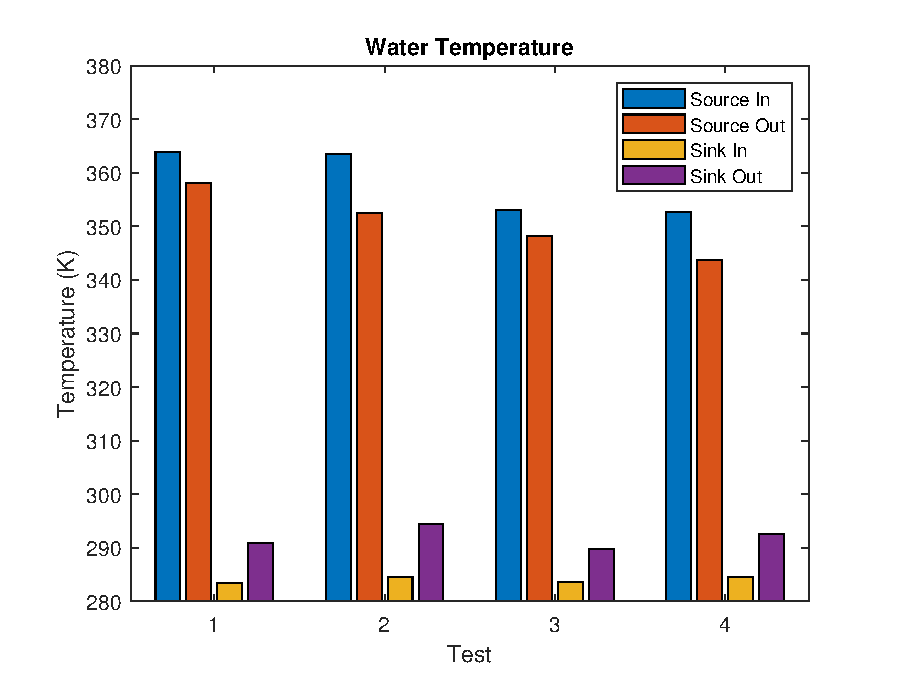
\includegraphics[width=\textwidth]{figures/VerificationWaterTemp02}
	%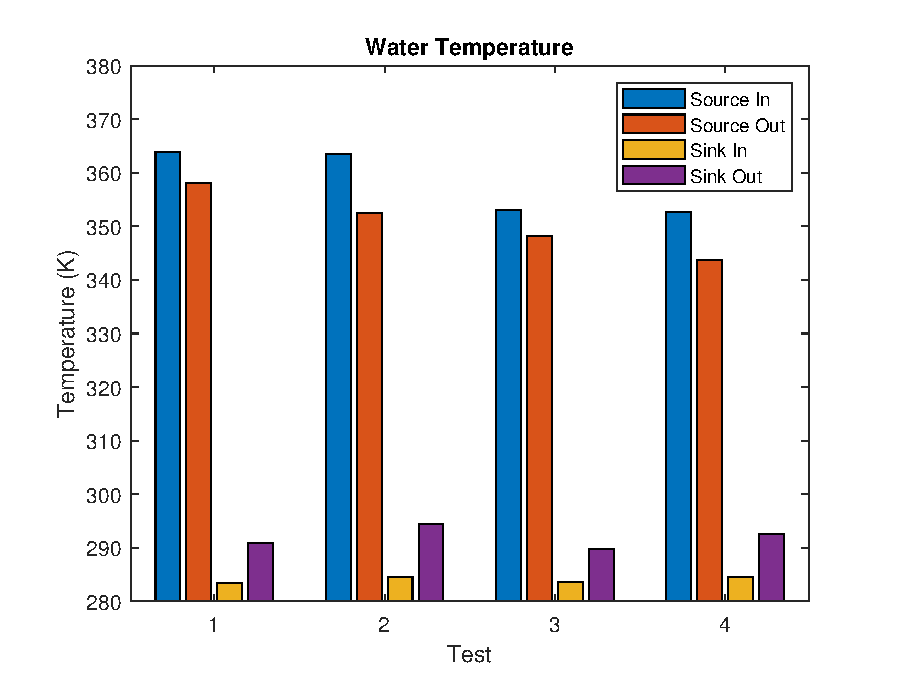
\includegraphics[width=0.5\textwidth]{figures/VerificationWaterTemp02}
	
	\caption{Comparison of source and sink inlet and outlet temperatures for the validation of the ORC prime power system model with an increased evaporator area. All tests assume a sink temperature of \SI{283}{\kelvin} (\SI{10}{\degreeCelsius}). Tests 1 \& 2 use a heat source temperature of \SI{364}{\kelvin} (\SI{91}{\degreeCelsius}), while tests 3 \& 4 use \SI{353}{\kelvin} (\SI{79}{\degreeCelsius}). Tests 1 \& 3 use a source flow rate of \SI{19}{\liter\per\second} and a sink flow rate of \SI{13}{\liter\per\second}, where as test 3 \& 4 use a source and sink flow rate of \SI{8}{\liter\per\second}.
	%The power setpoints of the four tests are \SIlist{27.5;40.0;30.8;42.0}{\kilo\watt}. Tests 1 \& 3 use the maximum power setpoint while also ensuring the working fluid fully evaporates in the evaporator. Tests 2 \& 4, use the maximum power setpoint while maintaining a stable simulation. 
	}
	%Psetpoint[2.75e4;4.0e4;3.08e4;4.2e4;]
	\label{fig:verificationWaterTemp02}
\end{figure}
\begin{figure}%[h]
	\centering
	\caption{Pressure-Enthalpy plot of R245-fa for ORC verification with an over sized evaporator area. Input tempetures and flow rates remain the same. 
	For tests 1 \& 2 $T_{source}$ is about \SI{364}{\kelvin} (\SI{195}{\degreeFahrenheit})
	while for 3 \& 4 $T_{source}$ is \SI{353}{\kelvin} (\SI{175}{\degreeFahrenheit}). 
	In all cases $T_{sink}$ is about \SI{283}{\kelvin} (\SI{50}{\degreeFahrenheit}). 
	The hot water flow rate for tests 1 \& 3 are \SI{18.9}{\liter\per\second} (\SI{300}{\gpm})
	and	\SI{7.6}{\liter\per\second} (\SI{120}{\gpm}) for test 2 \& 4. 
	The cold water flow rate for tests 1 \& 3 are \SI{12.6}{\liter\per\second} (\SI{200}{\gpm})
	and \SI{7.6}{\liter\per\second} (\SI{120}{\gpm}) for test 2 \& 4.}
	\label{fig:verifcation_ph02}
	
	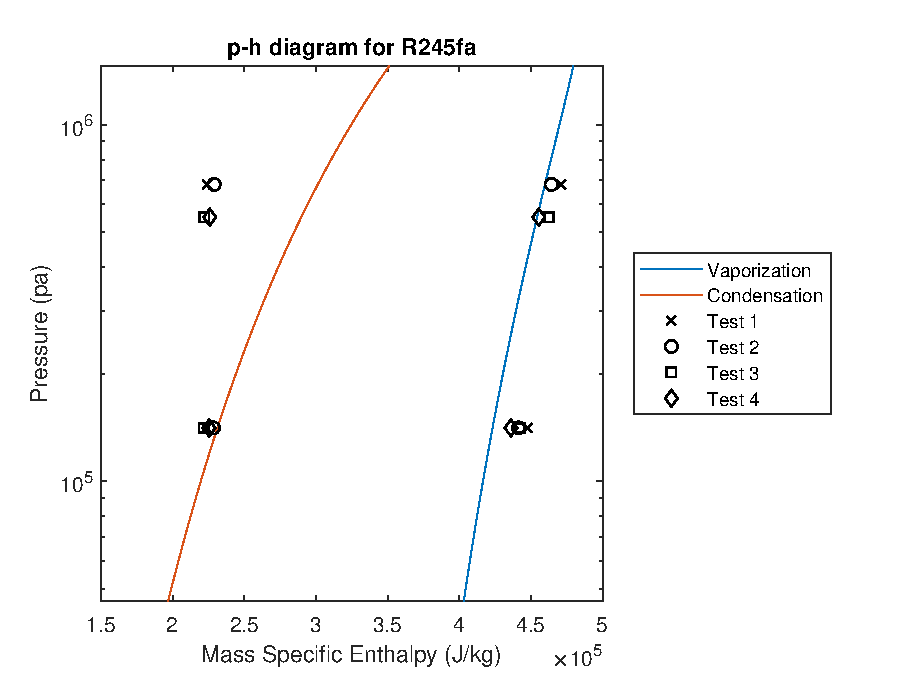
\includegraphics[width=\textwidth]{figures/VerificationPH02}
	%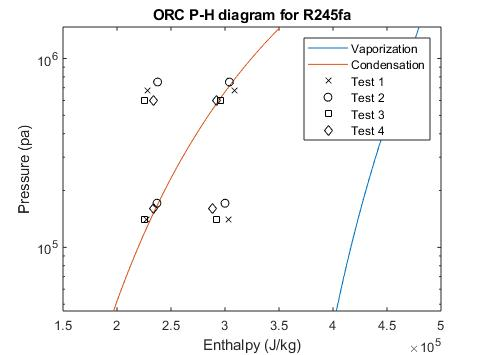
\includegraphics{figures/VerificationPH01}
\end{figure}

Under four different combinations of source and sink flow rates and temperatures, the gross output power of the model matched the measured values. However, given the assumed heat transfer area of the evaporator and condenser, the power consumed by the pump was calculated to be much greater than what was measured. Increasing the area of the evaporator such that it roughly matched the condenser greatly reduced the calculated power needed by the pump. However, this is not typical for ORCs. Generally condensers are sized larger than evaporators so the system can also feasibly use air to cool the working fluid. 
\clearpage

\section{Case Study Scenarios}
With the model validated the Greenfield and Brownfield scenarios can be simulated and analyzed. For the former, no electrical grid is currently present, while for the later there is existing electrical infrastructure. However, in the brownfield case the grid is not perfectly reliable. In the event of a grid outage, the microgrid should be capable of disconnecting and acting on its own. In both scenarios, the same generator impedances are used as in the validation simulations. 

\subsection{Greenfield Scenario --- Alaska}
This system is located approximately two hours north of Nome, Alaska on the western coast of the state. The hot water resource is drawn from the Pilgrim Hot Springs. The hot water is assumed to be drawn at a temperature of \SI{364.5}{\kelvin} (\SI{91.3}{\degreeCelsius}) and a flow rate of \SI{15.2}{\liter\per\second}. The hot water resource is fairly stable throughout the year. The low temperature water ranges from \SIrange{276.6}{281.6}{\kelvin} (\SIrange{3.5}{8.5}{\degreeCelsius}) at a flow rate of \SI{15.6}{\liter\per\second} to provide a heat sink \cite{Haselwimmer2013, AlaskaCenterforEnergyandPower2014}. Though the low temperature sink resource does vary in temperature with the seasons, the nearby geothermal activity keeps it liquid all year round.
%It is assumed the water is drawn in at atmospheric pressure.

The assumed working fluid is R245-fa, a typical refrigerant used by ORC manufacturers such as Electratherm, Clean Energy Technologies Inc., etc. The operating high and low pressure set points of the working fluid are \SIrange{570}{600}{\kilo\pascal} and \SIrange{130}{140}{\kilo\pascal}, respectively. The evaporator has a heat transfer area of \SI{37.8}{\meter\squared}, and an effective heat transfer coefficient of \SI{1500}{\watt\per\kelvin\per\meter\squared}. The condenser has an area of \SI{102.5}{\meter\squared}, but an effective heat transfer coefficient of \SI{1400}{\watt\per\kelvin\per\meter\squared}.

Four tests were conducted under different input conditions. Tests one and two use the warmer summer heat sink temperature, while tests three and four use the colder winter heat sink temperatures. Furthermore, tests one and three use the maximum power setpoint while also ensuring the working fluid fully evaporates in the evaporator, whereas in tests two and four, the power setpoint increased to the maximum value while maintaining a stable simulation. \autoref{fig:gfPower} compares the mechanical power, $P_{mech}$, the generator power, $P_{gen}$, inverter output power, $P_{out}$, and the electrical power consumed by the pump, $P_{pump}$ of the different tests. The working fluid mass flow rates, $\dot{m}$, are seen in \autoref{fig:gfFlow}. Finally, the heat flow rates of the evaporator and condenser, $\dot{Q}_{evap}$ and $\dot{Q}_{cond}$, are seen in \autoref{fig:gfHeat}.
\begin{figure}[p]
	\centering

	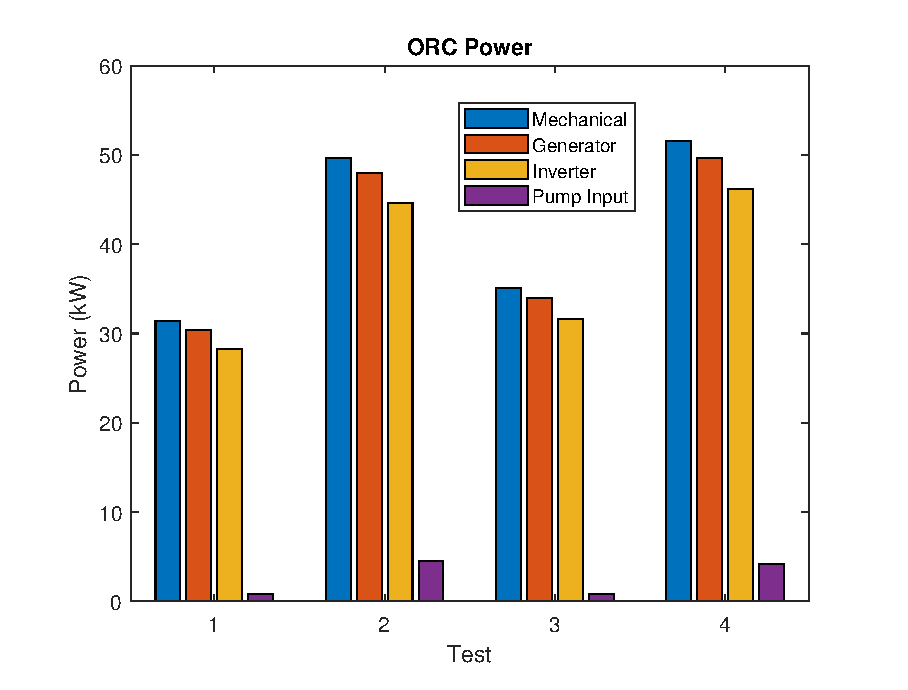
\includegraphics[width=\textwidth]{figures/gfPower}

	\caption{Comparison of mechanical power, generator power, inverter output power, and pump power consumption for the greenfield case of the ORC prime power system model. All tests assume a source temperature of \SI{364.5}{\kelvin} (\SI{91}{\degreeCelsius}), and source and sink flow rates of \SI{940}{\liter\per\minute}. Tests 1 and 2 use a heat sink temperature of \SI{281.6}{\kelvin} (\SI{8.5}{\degreeCelsius}), while tests 3 and 4 use \SI{276.6}{\kelvin} (\SI{3.5}{\degreeCelsius}). The power setpoints of the four tests are \SIlist{27.5;40.0;30.8;42.0}{\kilo\watt}. Tests 1 and 3 use the maximum power setpoint while also ensuring the working fluid fully evaporates in the evaporator. Tests 2 and 4 use the maximum power setpoint while maintaining a stable simulation. }
	%Psetpoint[2.75e4;4.0e4;3.08e4;4.2e4;]
	\label{fig:gfPower}
\end{figure}
\begin{figure}[p]
	\centering

	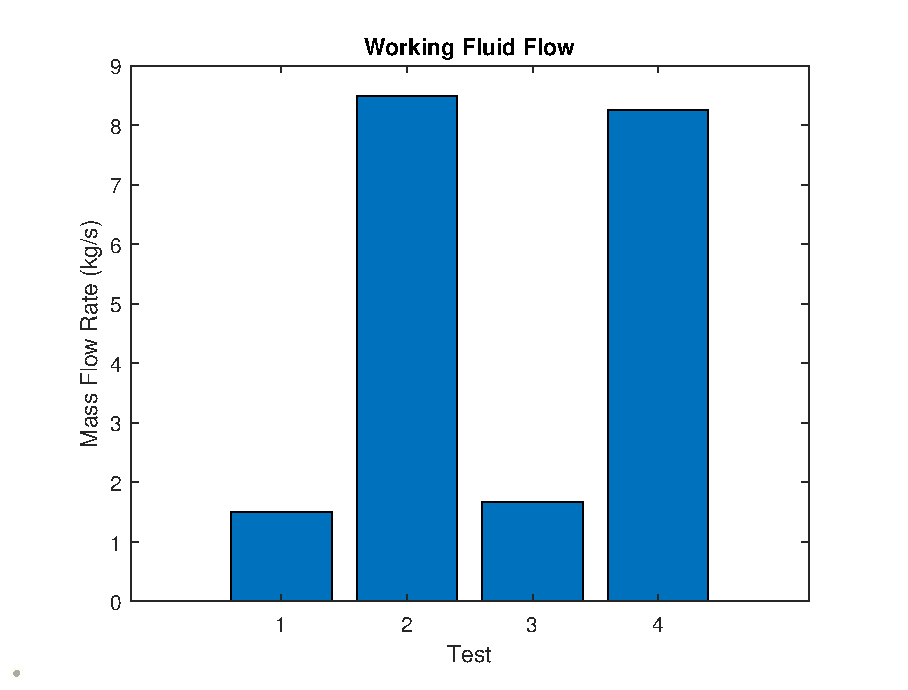
\includegraphics[width=\textwidth]{figures/gfFlow}

	\caption{Comparison of working fluid mass flow rates for the greenfield case of the ORC prime power system model. All test assume a source temperatures of \SI{364.5}{\kelvin} (\SI{91}{\degreeCelsius}), and source and sink flow rates of \SI{940}{\liter\per\minute}. Tests 1 and 2 use a heat sink temperature of \SI{281.6}{\kelvin} (\SI{8.5}{\degreeCelsius}), while tests 3 and 4 use \SI{276.6}{\kelvin} (\SI{3.5}{\degreeCelsius}). The power setpoints of the four tests are \SIlist{27.5;40.0;30.8;42.0}{\kilo\watt}. Tests 1 and 3 use the maximum power setpoint while also ensuring the working fluid fully evaporates in the evaporator. Tests 2 and 4 use the maximum power setpoint while maintaining a stable simulation. }
	%Psetpoint[2.75e4;4.0e4;3.08e4;4.2e4;]
	\label{fig:gfFlow}
\end{figure}
\begin{figure}[p]
	\centering

	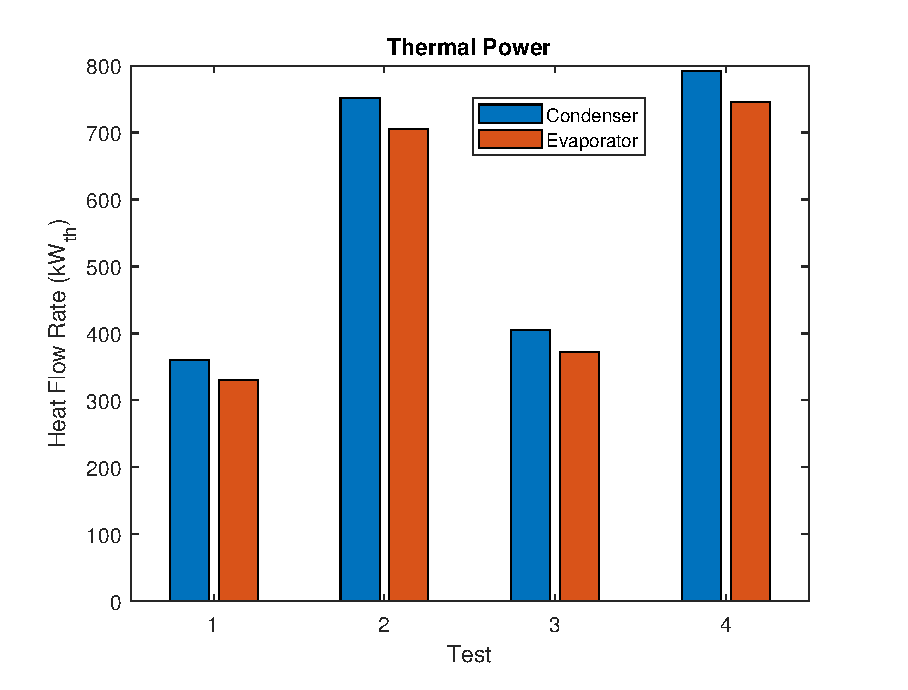
\includegraphics[width=\textwidth]{figures/gfHeat}

	\caption{Comparison among heat flow rates through the evaporator and condenser for the greenfield ORC prime power system model. All test assume a source temperatures of \SI{364.5}{\kelvin} (\SI{91}{\degreeCelsius}), and source and sink flow rates of \SI{940}{\liter\per\minute}. Tests 1 and 2 use a heat sink temperature of \SI{281.6}{\kelvin} (\SI{8.5}{\degreeCelsius}), while tests 3 and 4 use \SI{276.6}{\kelvin} (\SI{3.5}{\degreeCelsius}). The power setpoints of the four tests are \SIlist{27.5;40.0;30.8;42.0}{\kilo\watt}. Tests 1 and 3 use the maximum power setpoint while also ensuring the working fluid fully evaporates in the evaporator. Tests 2 and 4 use the maximum power setpoint while maintaining a stable simulation. }
	%Psetpoint[2.75e4;4.0e4;3.08e4;4.2e4;]
	\label{fig:gfHeat}
\end{figure}

Depending on the operator's tolerance of the state of the working fluid, the available gross output of the ORC prime power system can vary significantly. The gross output power of the inverter, $P_{out}$, the system can achieve while ensuring the working fluid fully vaporizes is \SIrange{28.3}{31.6}{\kilo\watt} throughout the year. In these cases the pump only needs to move about \SI{1.6}{\kilogram\per\second} consuming \SI{0.80}{\kilo\watt}. This yields a net output of \SIrange{27.5}{30.8}{\kilo\watt} before accounting for the power required for hot and cold water pumps. Heat is absorbed from hot water at a rate, $\dot{Q}_{evap}$, of \SIrange{361}{406}{\kilo\watt\textsubscript{th}} indicating a net efficiency of $\eta = 7.6\%$, where $\eta = \frac{P_{out}-P_{pump}}{\dot{Q}_{evap}}$.

More heat can be moved by increasing the working fluid flow rate yielding a greater gross output. For flow rates of around \SI{8.4}{\kilogram\per\second}, the gross output of the system is \SIrange{44.6}{46.2}{\kilo\watt}, with the greater end of the range occurring during the winter. Under these conditions the pump consumes about \SI{4.5}{\kilo\watt} cycling the working fluid, netting an output of \SIrange{40.1}{41.7}{\kilo\watt}. More power is being generated because heat is being transferred at a greater rate from the source, \SIrange{751}{792}{\kilo\watt\textsubscript{th}}, but the efficiency is lower at about 5.3\%.

The drop in efficiency from 7.6\% to 5.3\% as the working fluid flow rate increases can be understood by the plots in \autoref{fig:gf_themoplots}. The curves represent the dividing lines between pure liquid, pure gaseous, and the in-between state. The points represent the state of the working fluid between each block for the four different tests: low working fluid flow rate during summer, high flow rate during summer, low flow rate in winter, and high flow rate in winter. 
\begin{figure}%[h]
	\centering
	\caption{Thermodynamic plots of the simulated greenfield ORC plotting pressure against temperature, pressure against enthalpy, and temperature against entropy. All points assume a source temperatures of \SI{91}{\degreeCelsius}, and source and sink flow rates of \SI{940}{\liter\per\minute}. Winter sink temperatures are assumed to be \SI{3.5}{\degreeCelsius} while summer source temperatures are \SI{8.5}{\degreeCelsius}. High flow rate points have a working fluid mass flow rate of approximately \SI{8.4}{\kilogram\per\second}}
	\label{fig:gf_themoplots}
	
	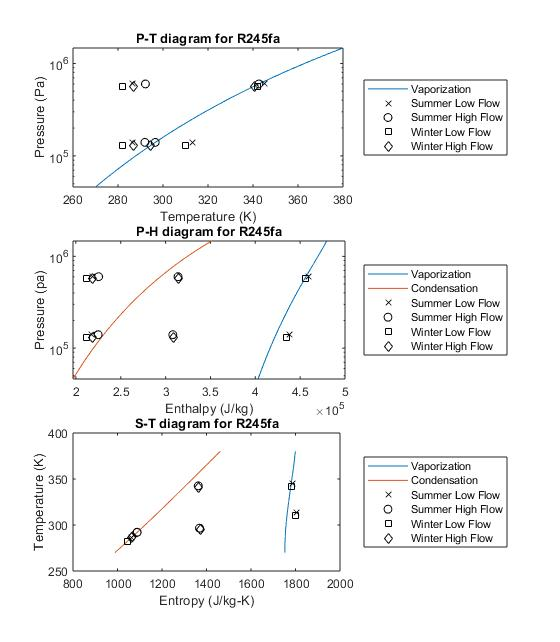
\includegraphics[width=\textwidth]{figures/GreenfieldThermoPlots}
	%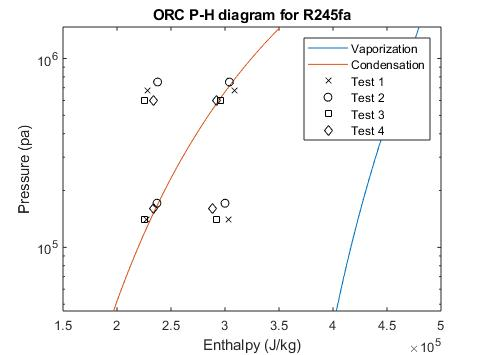
\includegraphics{figures/VerificationPH01}
\end{figure}

The first plot shows pressure (\si{\pascal}) versus temperature (\si{\kelvin}). A benefit of this plot is that it is easy to identify increases and decreases in both temperature and pressure as the working fluid moves through the cycle. However, this comes a cost of resolution in the liquid-vapor region. In this plot the vaporization and condensation curve overlap without representing the latent heat needed to change from one phase to the other. In this particular plot there are points in this area that are not discernible despite being at different energy levels. 

The second plot helps resolve this problem by plotting enthalpy (\si[per-mode=symbol-or-fraction]{\joule\per\kilogram}) on the x-axis instead of temperature. It can be seen that the low flow rate tests allow the fluid to fully become a gas and cross the vaporization curve. Since each \si{\kilogram} of fluid contains more energy, the turbine is able to operate more efficiently, even though more total energy is being extracted at higher flow rates.

The third and final plot of \autoref{fig:gf_themoplots} plots temperature (\si{\kelvin}) against mass specifc entropy (\si[per-mode=symbol-or-fraction]{\joule\per\kilogram\per\kelvin}). This shows the non-ideal isentropic transition of the pump and turbine. This is difficult to see for the pump because the points before and after the pump lie nearly on top of one another. Both the temperature and entorpy changed very little in the process. In the turbine, however, it is clearer. Ideally the points would drop straight down on this plot, but instead there is a slight increase in entropy due to the isentropic inefficiency, as expected from the 2\textsuperscript{nd} law of thermodynamics. 

The \SI{30.8}{\kilo\watt} output could be used to operate a greenhouse nearby during the winter. Assuming about \SI{1}{\kilo\watt} of power to supply the circulation fans and watering system, as well as LED lighting of 
%\SI{3.3}{\kilo\watt\per\meter\squared} \cite{Singh2015}
\SI{650}{\watt\per\meter\squared} \cite{Tamulaitis2005} for growing plants such as lettuce and radish, then a roughly \SI{45}{\meter\squared} greenhouse could be powered entirely off the ORC system. During the summer months fewer lights, if any, are needed to grow the plants due to the longer Alaskan days, therefore the lower available power would not be a problem.
\clearpage

\subsection{Brownfield Scenario --- Iceland}
Bergsta$\eth$ir, Iceland is located inland east of Reykjavík. The hot water resource is drawn at a flow rate of about \SI{6}{\liter\per\second} from below the surface to a holding tank before being distributed to the homes for heating. While sitting in this tank, the water is approximately \SI{}{\kelvin} (\SI{95}{\degreeCelsius}). Nearby there is a \SI{}{\kelvin} (\SI{5}{\degreeCelsius}) stream which can be drawn from in order provide a low temperature sink fluid.

The working fluid is also assumed to be R245-fa. The operating high and low pressure set points of the working fluid are \SI{600}{\kilo\pascal} and \SI{140}{\kilo\pascal}. The evaporator has a heat transfer area of \SI{37.83}{\meter\squared}, and an effective heat transfer coefficient of \SI{1500}{\watt\per\kelvin\per\meter\squared}. As before, it is usual in commercial ORC systems for the condenser to have a greater area to allow for the option of air cooling. In this case the condenser has an area of \SI{37.83}{\meter\squared}, and an effective heat transfer coefficient of \SI{1400}{\watt\per\kelvin\per\meter\squared}. The pump and its driving motor are assumed to have efficiencies of 70\% and 90\%, respectively. The turbine is assumed to have a mechanical efficiency of 78\% for the operating conditions.
%, while the input parameters of the generator can be seen in Fig X. 
The inverter used to convert the unregulated AC output of the self excited induction generator to a regulated 60 Hz is assumed to have an efficiency of 93\%.

Under these conditions, the model predicts an ORC prime power system to produce \SI{31.7}{\kilo\watt} of mechanical power, \SI{30.8}{\kilo\watt} from the induction generator, and a gross electrical output of \SI{28.6}{\kilo\watt} from the grid forming inverter, plotted in \autoref{fig:bfPower}. To circulate the working fluid, the pump needs to consume \SI{0.8}{\kilo\watt}, resulting in \SI{27.8}{\kilo\watt} available for other devices on the microgrid. Unfortunately, this is insufficient for the desired application of this system;  running two 15 kW motors used to distribute the hot water for home heating. Additionally, this does not even take into account the pump needed to collect the low-temperature stream water for the low temperature sink.
\begin{figure}[h]
	\centering

	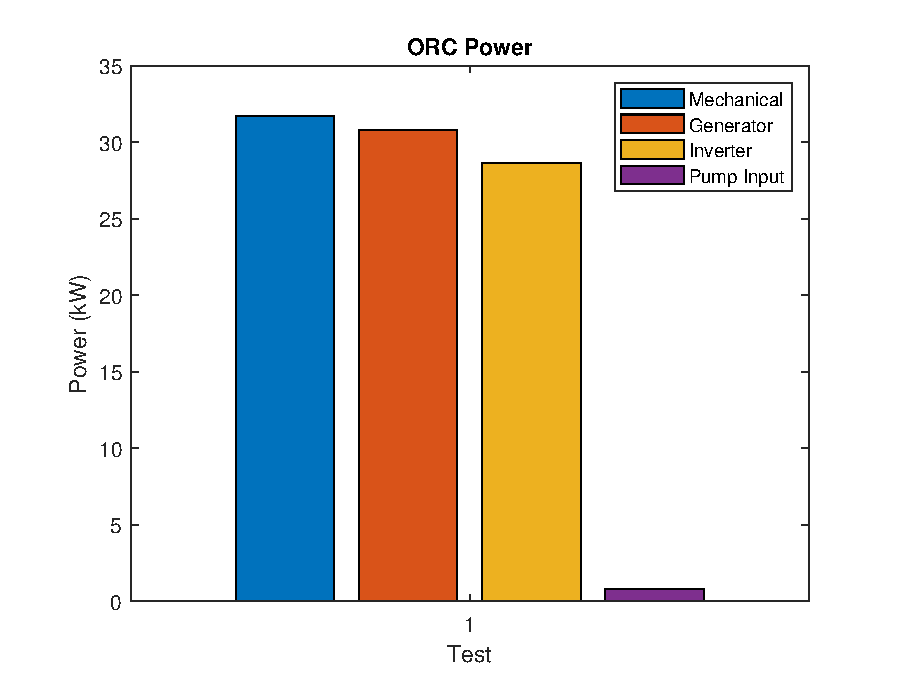
\includegraphics[width=\textwidth]{figures/bfPower}

	\caption{Comparison of mechanical power, generator power, inverter output power, and pump power consumption for the brownfield case of the ORC prime power system model. The test assumes a source temperature of \SI{368}{\kelvin} (\SI{95}{\degreeCelsius}) and a sink temperature of \SI{278}{\kelvin} (\SI{5}{\degreeCelsius}). The source is assumed to flow at a rate of \SI{6}{\liter\per\minute} while the sink flows at \SI{7}{\liter\per\minute}. }
	%Psetpoint[2.75e4;4.0e4;3.08e4;4.2e4;]
	\label{fig:bfPower}
\end{figure}

\autoref{fig:bf_themoplots} shows similar thermodynamic plots as the greenfield scenario. The top right point of each plot represents the state of the working fluid as it is leaving the evaporator before entering the expander. It can be seen that this point lies on the vaporization curve. This means if the working fluid mass flow rate were to increase in order to get more power out, then the fluid would not fully vaporize and the expander efficiency assumption would no longer be valid.
If the amount of heat transferred could be increased, then it's possible the working fluid flow rate could increase as well while maintaining full vaporization. 
\begin{figure}[h]
	\centering

	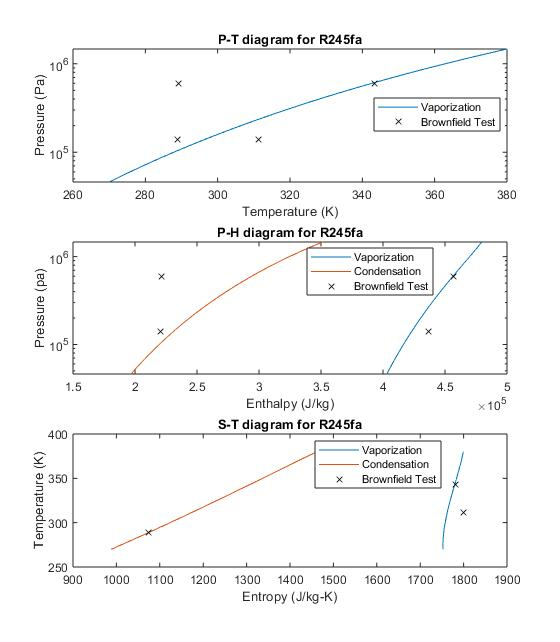
\includegraphics[width=\textwidth]{figures/BrownfieldThermoPlots}
	%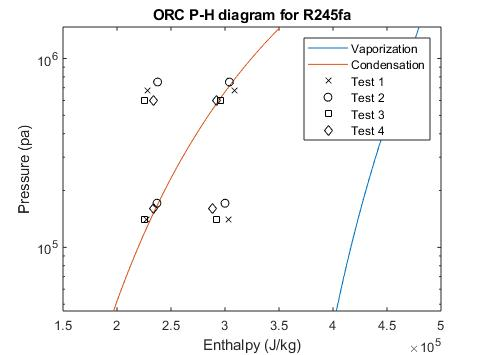
\includegraphics{figures/VerificationPH01}
	\caption{Thermodynamic plots from the simulated brownfield ORC prime power system plotting pressure against temperature (top), pressure against mass specific enthalpy (middle), and temperature against mass specific entropy (bottom). Source temperature and flow rate are assumed to be \SI{368}{\kelvin} (\SI{95}{\degreeCelsius}) and \SI{6}{\liter\per\second}. Sink temperature and flow rate are assumed to be \SI{278}{\kelvin} (\SI{5}{\degreeCelsius}) and \SI{7}{\liter\per\second}.}
	\label{fig:bf_themoplots}
\end{figure}

\cleardoublepage
\chapter{Conclusions and Future Work}
\label{ch:conclusion}

The goal of this thesis was to explore a viable and affordable method of incorporating geothermal energy as a prime power source to form a microgrid using an organic Rankine system. Low temperature geothermal sites were looked at specifically because such sites can be found within Alaska and similar environments which are not currently fully utilized. To achieve the goal, a model was developed to simulate the thermodynamic and electrical processes of the ORC and the SEIG. Next, two different systems were examined: a greenfield site with minimal existing infrastructure and a brownfield site that is already connected to an electric grid for pump power. 

\section{Model Validation}
In order to verify that the model approximates reality, a Electratherm Green Machine was simulated under testing conditions. These values were compared to the results of a Green Machine test at the University of Alaska Fairbanks. There were some difficulties in re-creating exact conditions because some values were not precisely recorded. For example, operating ranges for the high and low pressures of the working fluid were stated, but specific measurements were not included. 
Other values, were assumed while sizing the ORC for the test but not measured after the installation because the report was interested in the performance of the whole unit rather than modeling it. These values include the heat transfer coefficients and areas of the heat exchangers, as well as the isentropic efficiencies of the pump and expander.
% area/U discrpencies

Despite the differences in these parameters between the model and the report, the model was still validated based on the general trends in the output power. Higher source fluid temperatures yield more power. Greater mass flow rates of the source and sink similarly provide a greater output power, though this is limited by the parameters of the heat exchangers. Additionally, it was shown that a larger heat exchanger area will transfer heat at a greater rate than a smaller area, while accounting for mass flow rates. These patterns and trends follow what is expected for an organic Rankine cycle system.

\section{Greenfield}
%It was shown that output of an ORC could produce a net output of around \SIrange{27.5}{30.8}{\kilo\watt} over the course of the year. This is due to a steady temperature hot water resource and a cold water sink that varies over seasons but remains liquid. 
The greenfield simulations demonstrated the expected increase of available power output during winter months. 
According to the model, even more power could be produced by increasing the mass flow rate of the working fluid. However, this assumes the isentropic efficiency of the turbine expander is equal in the two cases, which is unlikely. The additional mass means the fluid does not fully vaporize, which is not typical for ORC systems because the efficiency is not constant under all conditions. 

While the available power gained by increasing the flow rate of the working fluid is limited by the vaporization, that flow rate limit could be increased by also increasing the flow rates of the source and sink fluids. Hypothetically, the higher flow rates mean larger pumps and heat exchangers must be used for the system, increasing the total cost, but that should be offset by the increase in output power. Realistically, though, only so much hot water can be drawn from geothermal resources before the source temperature begins to drop. This can be alleviated by re-injecting the source effluent up to a point. However, the model assumes the resources are steady, and if the flow rates are increased too much, that assumption would no longer be valid.


\section{Brownfield}
In the brownfield case study it was shown the ORC could not produce enough electrical power to drive the district heating loop pumps from the inverter as a prime power source.
%The expected net power produced by an ORC for a brownfield system is \SI{27.8}{\kilo\watt}, just under the desired \SI{30}{\kilo\watt} needed to drive the district heating pumps.
However, there was sufficient power produced, but due to inefficiencies and parasitic loads there was not enough remaining to power everything. 
%The gross electrical power produced by the generator before inverter losses is just shy of \SI{30.8}{\kilo\watt}. 
This indicates there may be enough power from the local resource to operate the district heating system while the electrical grid is active and capable of regulating the frequency and voltage of the induction generator. However, the whole system would still go down during a power outage and the diesel generators would still need to be used to give the community heat, albeit with lower fuel consumption than without the ORC system.

One possible solution is to increase the size of the evaporator area. This could allow the more heat to flow from the water to the working fluid, meaning the more fluid could be moved while still fully vaporizing. Unfortunately, the cost of the system would go up as well due to larger heat exchanger.

%check the mech power produced
Another option could be to bypass electrical conversion entirely, eliminating several inefficiencies along the way. The simulated ORC produced more mechanical power than electrical, and the mechanical load to drive the pumps is actually less than the rated electrical load.
%The simulated ORC produced about \SI{31.7}{\kilo\watt} of mechanical power, and the \SI{30}{\kilo\watt} district heating pumps actually need slightly less mechanical power to operate.
A system could be developed to connect the ORC expander to a mechanical pump to drive the district heating loop. Depending on the design, this could be done with a direct coupling or through a gearbox of some kind. Of course, other inefficiencies would be introduced and controlling the flow would be challenging, but it might be worth further examination.

\section{Future Work}
One improvement that the model would need before it can be more widely is a user friendly graphical interface. Currently, an MATLAB script is run in order to initialize all the input variables and parameters, then the Simulink simulation can be run, and finally a second script is run to generate the plots. Combining some of these steps into a graphical user interface, this model could be more readily utilized by others. In addition to the interface, there are other potential improvements relating the thermal, electrical, and transient aspects of the model.

\subsection{Thermal Model}
As described previously, 
%more heat was transferred through the heat exchangers in the model than what was measured in actual testing of an ORC device. A possible explanation is that 
the model is perfectly efficient at transferring the heat and none is lost to the ambient environment. In reality, fluid in the heat exchangers, pumps, expanders, and pipes will experience some amount of heat loss or gain to the surrounding area. Furthermore, the model only calculated pressure changes across the pump and expander, where as fluids in actual systems will see some pressure drops through each component. The overall accuracy of the model could be improved by accounting for this additional routes of heat flow and pressure changes.

Another implementation that could improve system performance is an optional pre-heater that several commercial systems already use. This heat exchanger is inserted in the loop between the pump and evaporator on the high pressure side effectively increasing the area of the evaporator. Sometimes the pre-heater uses a different heat source from the primary source. Even the heat of the working fluid coming off of the expander before flowing through the condenser could be used. This allows the system to recycle some of the heat that was not converted into mechanical energy letting it operate at a slightly higher efficiency at the cost of an additional component.

\subsection{Electrical Model}
The microgrids simulated as a part of this project only included squirrel cage induction generators because they are relatively inexpensive to build and maintain, and are therefore commonly used in commercial ORC systems. They are not, however, ubiquitous. It would be beneficial to include models of additional generator types such as DC or permanent magnet synchronous machines. This would allow the user to compare systems made by different manufacturers which use various generator technologies.
%various inverter models
%add storage

\subsection{Transient Model}
This model was designed to examine steady-state results. It looks at the energy balance of each component to simulate how they interact over long term. This means it is unable to accurately capture transient dynamics after a change in load, temperature, or flow rate. Each of those fluctuations can occur at different time scales and effect the system dynamics differently. It is important to know the system is capable of providing primary power while maintaining grid frequency and voltage under those different perturbations.

\section{Final Thoughts}
Overall, this thesis demonstrated that for remote greenfield microgrids, modest loads can be primarily powered off of these low temperature geothermal organic Rankine cycles. At the Pilgrim hot springs in Alaska, a small greenhouse could be designed and built to operate in the winter using LED grow lights. This could provide a source of fresh local vegetables to the nearby community of Nome all year. 

For brownfield microgrids, there is less flexibility because the loads are already present and cannot be designed around the available source. For the village of Bergsta$\eth$ir, Iceland the geothermal ORC prime power system presented here could not, on its own, fully supply the existing district heating system. The ORC could, however, provide most of the necessary power, meaning the a significant portion of the diesel fuel used to operate the district heating system during power outages could be displaced.

\cleardoublepage



\bibliographystyle{ieeetr}
\bibliography{NG_bib}

\end{document}
